                 %% ****** Start of file template.aps ****** %
%%
%%
%%   This file is part of the APS files in the REVTeX 4 distribution.%!TEX encoding = UTF-8 Unicode
%%   Version 4.0 of REVTeX, August 2001
%%
%%
%%   Copyright (c) 2001 The American Physical Society.
%%
%%   See the REVTeX 4 README file for restrictions and more information.
%%
%
% This is a template for producing manuscripts for use with REVTEX 4.0
% Copy this file to another name and then work on that file.
% That way, you always have this original template file to use.
%
% Group addresses by affiliation; use superscriptaddress for long
% author lists, or if there are many overlapping affiliations.
% For Phys. Rev. appearance, change preprint to twocolumn.
% Choose pra, prb, prc, prd, pre, prl, prstab, or rmp for journal
%  Add 'draft' option to mark overfull boxes with black boxes
%  Add 'showpacs' option to make PACS codes appear
%  Add 'showkeys' option to make keywords appear
\documentclass[aps,prstab,twocolumn,superscriptaddress]{revtex4}
\usepackage{graphicx}
\usepackage{url}
%\usepackage[center]{caption2}
\usepackage[colorlinks,linkcolor=blue,anchorcolor=blue,citecolor=green]{hyperref} % hyper reference to contents 
%\documentclass[aps,prl,preprint,superscriptaddress]{revtex4}
%\documentclass[aps,prl,twocolumn,groupedaddress]{revtex4}

% You should use BibTeX and apsrev.bst for references
% Choosing a journal automatically selects the correct APS
% BibTeX style file (bst file), so only uncomment the line
% below if necessary.
\bibliographystyle{apsrev}
\newcommand{\opal}{\textsc{OPAL}}
\newcommand{\opalt}{\textsc{OPAL-t }}
\newcommand{\opalcycl}{\textsc{OPAL-cycl}}
\newcommand{\opalmap}{\textsc{OPAL-map }}
\newcommand{\opalenv}{\textsc{OPAL-envelop}}

\newcommand{\mad}{\textsc{mad }}
\newcommand{\madnine}{\textsc{mad9 }}
\newcommand{\madninep}{\textsc{mad9p }}
\newcommand{\madeight}{\textsc{mad8 }}

\newcommand{\classic}{\textsc{classic }}
\newcommand{\hfifepart}{\textsc{H5Part }}
\newcommand{\hfifefe}{\textsc{H5FED }}

\renewcommand{\epsilon}{\varepsilon} 
\renewcommand{\vec}[1]{{\bf #1}} 
\newcommand{\dt}[1]{\frac{\partial #1}{\partial t}}
\newcommand{\dtt}[1]{\frac{\partial^2 #1}{\partial t^2}}
\newcommand{\dtvec}[1]{\frac{\partial {\mathbf #1}}{\partial t}}
\newcommand{\dttvec}[1]{\frac{\partial^2 {\mathbf #1}}{\partial t^2}}
\newcommand{\rot}{\vec{\nabla} \wedge }
\renewcommand{\div}{\vec{\nabla} \cdot }

\def\vec#1{\mathbf{#1}}
\def\vecg#1{\boldsymbol{#1}}
\def\norm#1{\| #1 \|} 
\def\tr{^{\!\top}}

\def\curl{{\bf curl}\,}
\def\curlp{{\rm curl}_p\,}
\def\div{{\rm div}\,}
\def\grad{\nabla}
\def\gradp{\nabla_p}
\def\dotp#1#2{\langle#1,#2\rangle}
\def\eps{\varepsilon}

\newcommand{\mat}[1]{\ensuremath{\boldsymbol{#1}}}
\newcommand{\vect}[1]{\ensuremath{\mathbf{#1}}}
\newcommand{\iprod}[2]{\ensuremath{\langle#1,#2\rangle}}
\newcommand{\abs}[1]{\ensuremath{|#1|}}

\newcommand{\Nedelec}{N\'{e}d\'{e}lec}

\newcommand{\id}[1]{\structure{#1}}

\newcommand {\Co}{{\mathbb{C}}}
\newcommand {\Int}{{\mathbb{Z}}}
\newcommand {\Nat}{{\mathbb{N}}}
%
%
\newcommand {\Hcurl}{{H(\mathbf{curl};\Omega)}}
\newcommand {\Hocurl}{{H_0(\mathbf{curl};\Omega)}}
\newcommand {\Hdiv}{{H(\mathrm{div};\Omega)}}
\newcommand {\Hodiv}{{H_0(\mathbf{div};\Omega)}}
%
\renewcommand {\Re}{{\rm I \kern-2pt R}}
\newcommand{\vc}[1]{\mbox{\boldmath $#1$}}
\newcommand {\RM}[1]{\mathrm{#1}}


\newcommand{\bs}[1]{\mathbf #1}
\renewcommand{\baselinestretch}{2.0}
\begin{document}

% Use the \preprint command to place your local institutional report
% number in the upper righthand corner of the title page in preprint mode.
% Multiple \preprint commands are allowed.
% Use the 'preprintnumbers' class option to override journal defaults
% to display numbers if necessary
%\preprint{}

%Title of paper
%\title{OPAL-cycl: A Parallel PIC code Including Neighboring Bunch Effects in High Intensity  Cyclotrons
\title{Beam Dynamics in High Intensity Cyclotrons Including Neighboring Bunch Effects Part 1: Model, Implementation and Validation}
%\title{Numerical Study of Beam Dynamics in High Intensity Cyclotrons Including Neighboring Bunch Effects}
%\title{OPAL-cycl: A Parallel PIC code Including Neighboring Bunch Effects in High Intensity Cyclotrons}

% repeat the \author .. \affiliation  etc. as needed
% \email, \thanks, \homepage, \altaffiliation all apply to the current
% author. Explanatory text should go in the []'s, actual e-mail
% address or url should go in the {}'s for \email and \homepage.
% Please use the appropriate macro foreach each type of information

% \affiliation command applies to all authors since the last
% \affiliation command. The \affiliation command should follow the
% other information
% \affiliation can be followed by \email, \homepage, \thanks as well.
\author{J. Yang}
\email{yangjianjun00@mails.tsinghua.edu.cn}
%\homepage[]{Your web page}
%\thanks{}
\affiliation{China Institute of Atomic Energy, Beijing, 102413, China}
\affiliation{Paul Scherrer Institut, Villigen, CH-5234, Switzerland}
\affiliation{Tsinghua University, Beijing, 100084, China}
\author{A. Adelmann}
\email{andreas.adelmann@psi.ch}
\author{M. Humbel}
\author{M. Seidel}
\affiliation{Paul Scherrer Institut, Villigen, CH-5234, Switzerland}
\author{T. Zhang} 
\affiliation{China Institute of Atomic Energy, Beijing, 102413, China}

%Collaboration name if desired (requires use of superscriptaddress
%option in \documentclass). \noaffiliation is required (may also be
%used with the \author command).
%\collaboration can be followed by \email, \homepage, \thanks as well.
%\collaboration{}
\noaffiliation

\begin{abstract}
Space charge effects play an important role in high intensity cyclotrons, as the most important collective effect. 
For high intensity cyclotrons with small turn separation, single bunch space charge effects are not the only contribution. 
The interaction of radially neighboring bunches is also present but its effects have not yet been investigated in greater detail.
In this paper, for the first time, a new PIC based self-consistent numerical simulation model is presented, 
which covers neighboring bunch effects and is implemented in a three-dimensional object-oriented parallel code \opalcycl,
a flavor of the \opal \  framework. 
We present simulation results from the PSI 590\,MeV Ring cyclotron in the light of the ongoing high intensity upgrade program,
with the goal of 1.8\,MW CW beam power on target.
\end{abstract}

% insert suggested PACS numbers in braces on next line
\pacs{}
% insert suggested keywords - APS authors don't need to do this
%\keywords{}

%\maketitle must follow title, authors, abstract, \pacs, and \keywords
\maketitle

% body of paper here - Use proper section commands
% References should be done using the \cite, \ref, and \label commands
%\section{}
% Put \label in argument of \section for cross-referencing
\section{INTRODUCTION \label{intro}}
%1.Brief review of history of space charge effects in cyclotron. 
Since the invention of the first classic cyclotron several decades ago, the higher beam intensity is always required  
to provide more powerful tools for many new scientific applications, such as Spallation Neutron Source (SNS)
and Accelerator Driven System (ADS).
In high intensity cyclotrons, space charge effects play an important role for the following reasons.
Firstly, longitudinal focusing is missing in cyclotrons and the disruptive longitudinal space charge force causes additional acceleration for 
head particles and deceleration for tail particles, which may results in an increase of the energy spread. Secondly, there is a strong 
radial-longitudinal coupling which is influenced by non-linear radial and longitudinal space charge forces. 
Lastly, the space charge force can reduce the vertical tune and increase the vertical beam size, which can cause major beam loss when 
it goes beyond the aperture of the accelerator, and therefore limits the maximal beam current \cite{Baartman:1}.

The non-linear space charge effects in cyclotrons are complex also because of the complicated magnetic topology (reference trajectory with non constant
curvature). Typically there are two approaches 
to deal with the mentioned complexity: one is the approximation with analytic and semi-analytic models which are cheap to compute. With such models we can obtain a qualitative  
understanding of the problem. %, but they can not give out accurate solutions.
In the past, a number of models have been developed based on this philosophy, such as the Sector Model, Disk Model, Sphere Model and the so called Needle Model \cite{Gordon:1,Joho:1,Adam:1,Adam:2}. 
Another more accurate approach is numerical simulation with macro-particles. In this field, typically two different technologies were used to 
solve space charge fields: Particle-Particle (P-P) methods \cite{Li:1} and Particle-Mesh (P-M) methods \cite{Ada:1,Poz:1}. In P-P methods, the field imposed on 
a given particle is obtained by directly summing up the contributions of all other particles at this position. Limited by its low computation efficiency ($\mathcal{O}(n^2)$ with $n$ denoting the number of simulation particles), 
it is impossible to utilize these methods for large scale particles problems (above 1\,million), even on current top speed supercomputers. In contrary, P-M methods
calculate fields indirectly based on discrete grid domain. Due to its high efficiency and high precision, P-M based Particle-In-Cell (PIC) methods\cite{Hockney:1} 
are widely used in parallel macro-particles simulation codes for different types of accelerators and beam lines \cite{Ada:1,Qiang:1,Gala:1,Grote:1,Huang:1} 
as well as many other areas of computational science, thanks to the development of parallel computation technology during recent years. Therefore, parallel PIC methods are 
chosen in our study on beam dynamics of high intensity cyclotrons.

For high intensity cyclotrons with small turn separation, single bunch space charge effects are not the only contribution. 
Along with the steady increase of beam current, the mutual interaction of neighboring bunches in radial direction 
becomes more and more important, especially at large radii where the distances between neighboring bunches get increasingly small, and even overlap can occur.
One good example is PSI 590\,MeV Ring cyclotron \cite{Mike:1} with a production current of about 2\,mA in CW operation and a beam power on target of approximately 1.2\,MW.
An ambitious upgrade program for the PSI Ring cyclotron is funded and in progress, aiming for 1.8\,MW CW beam power on target. 
The concept involves replacing four aluminum resonators by new copper resonators with peak voltages
increasing from about 0.7\,MV to above 0.9\,MV. After the planed upgrade, the total turn number can be significantly reduced, e.g. from more than 200 turns to less than 
170 turns.
In consequence the turn separation is increased, but remains at the same order of magnitude as the radial bunch size, as shown in Fig.\,\ref{fig:TuneSep} (The main cavity voltage is 0.735 and 0.9\,MV respectively and
      flat-top is 11.2$\%$ of main voltage).
Therefore, when the beam current increases from 2\,mA to 3\,mA, 
the mutual space charge effects between radially neighboring bunches will have more impact on the beam dynamics and need to be considered seriously.
Another example is the 100\,MeV, compact cyclotron CYCIAE-100 under construction at CIAE \cite{Zhang:1}. Although its beam current is only 200\,$\mu$A to 500\,$\mu$A,
because of the small energy gain per turn (about 200\,keV), the turn separation is far smaller than the beam size at outer radii (at the extraction, $\Delta R = 1.5\RM{\,mm}$) and
multiple bunches will overlap.

Because of the complexity of the problem, it is impossible to evaluate neighboring bunch effects precisely and self-consistently by explicit 
analytic expressions. However, the fast developing computer hardware and high performance computation (HPC) makes it possible to 
treat this problem in greater detail. To our knowledge, very few research efforts have been done on neighboring bunch effects, the only published work so far is the one of   
E.Pozdeyev's work \cite{Poz:1}. He introduced ``rigid auxiliary bunches'' in his serial code CYCO which uses the azimuthal angle as the independent variable. 

In Section II and III, a new PIC based self-consistent numerical simulation model which covers neighboring bunch effects is presented. 
Section IV describes our three-dimensional object-oriented parallel simulation code \opalcycl, a flavor of the \opal \  framework. 
The results of performance testing and code benchmarking are presented in Sec.V, and followed by its applications on PSI 590\,MeV Ring cyclotron in VI. 

    
  \begin{figure}
    {\includegraphics[width=8cm,trim=2.5cm 2.5cm 2.5cm 2.5cm]{figures/R_dR_Ring.pdf}}
    {\includegraphics[width=8cm,trim=2.5cm 2.5cm 2.5cm 2.5cm]{figures/Turn_dR_Ring.pdf}}
    \caption{Comparison of calculated turn separation for centroid particles before (red line) and after (blue line) upgrade of the PSI Ring Cyclotron.}
    %The result is given by single particle tracking using \opalcycl. Noting that it is increased by about 3\,mm by the fringe field effects at extraction point}
    \label{fig:TuneSep}
  \end{figure}

\section{BASIC EQUATIONS AND PHYSICAL MODEL }
%1.Coordinates frame, basic equation of particle motions, time integrator, external field interpolation and treatment.
%2.Brief introduction of PIC methods, such as FFT, Green function, CIC scheme.

In our Cyclotrons and beam lines, the collision between particles can be neglected because the   typical bunch densities are low.
In time domain, the general equations of motion of charged particle in electromagnetic field can be expressed by
\begin{equation}\label{eq:motion}
  \frac{d\bs{p}(t)}{dt}  = q\left(c\bs{\beta}\times \bs{B} + \bs{E}\right), \nonumber \\
\end{equation}
where $m_0, q,\gamma$ are rest mass, charge, relativistic factor, $\bs{p}=m_0 c \gamma \bs{\beta}$ momentum of a particle respectively, 
$c$ light velocity, $\bs{\beta}=(\beta_x, \beta_y, \beta_z)$ normalized velocity vector. If $\bs{p}$ is normalized by $m_0c$, 
Eq.\,(\ref{eq:motion}) can be written in Cartesian coordinates as 
\begin{eqnarray}\label{eq:motion2}
  \frac{dp_x}{dt} & = & \frac{q}{m_0c}E_x + \frac{q}{\gamma m_0}(p_y B_z - p_z B_y),    \nonumber \\
  \frac{dp_y}{dt} & = & \frac{q}{m_0c}E_y + \frac{q}{\gamma m_0}(p_z B_x - p_x B_z),   \\
  \frac{dp_z}{dt} & = & \frac{q}{m_0c}E_z + \frac{q}{\gamma m_0}(p_x B_y - p_y B_x).    \nonumber 
\end{eqnarray}
The evolution of the beam's distribution function $ f(\bs {x},c\bs{\beta},t)$ can be expressed by collisionless Vlasov equation:
\begin{equation}\label{eq:Vlasov}
  \frac{df}{dt}=\partial_t f + c\bs{\beta} \cdot \nabla_x f +q(\bs{E}+ c\bs{\beta}\times\bs{B})\cdot \nabla_{c\bs{\beta}} f  =  0, 
\end{equation}
where $\bs{E}$ and $\bs{B}$ includes both external applied fields, space charge fields and other collective effects such that wake fields
\begin{eqnarray}\label{eq:Allfield}
  \bs{E} & = & \bs{E_{\RM{ext}}}+\bs{E_{\RM{sc}}}+\bs{E_{\RM{wake}}}, \nonumber\\    
  \bs{B} & = & \bs{B_{\RM{ext}}}+\bs{B_{\RM{sc}}}+\bs{B_{\RM{wake}}}.
\end{eqnarray}
In order to model a cyclotron, the external electromagnetic fields are given by measurement or by numerical calculations. 
Wake fields tightly depend on the structure of the vacuum chamber and are neglected in this study. 

% In the working area of a cyclotron, the boundary conditions are open on both the radial and azimuthal directions, and 
% on vertical direction it is smooth and flat, therefore $\bs{E_{wake}}$ and $\bs{B_{wake}}$ are negligible when compare with space charge fields.
The space charge fields can be obtained
by a quasi-static approximation. In this approach, the relative motion of the particles is non-realitivistic in the beam rest frame, so self-induced magnetic field is practically absent and the electric field can be computed by solving Poisson equation
\begin{equation}\label{eq:Poisson}
  \nabla^{2} \phi(\bs{x}) = - \frac{\rho(\bs{x})}{\varepsilon_0},
\end{equation}
where $\phi$ and $\rho$ are the electrostatic potential and the spatial charge density in the beam rest frame. The electric field can then be calculated by
\begin{equation}\label{eq:Efield}
  \bs{E}=-\nabla\phi.
\end{equation}
This electric field can be transformed to yield both the electric and the magnetic fields required in Eq.\,(\ref{eq:Allfield}) by means of a Lorentz transformation.
In cyclotron the contribution of image charges and currents should be only small effects compared to the direct space charges \cite{Baartman:1}, so it should be a good approximation to use 
open boundary conditions. 

The combination of Eq.\,(\ref{eq:Vlasov}) and Eq.\,(\ref{eq:Poisson}) constitutes the Poisson-Vlasov equation system. 
Parallel PIC methods is a highly efficient approach of solving Poisson-Vlasov equations in large-scale simulations. 

%In PIC methods, firstly a 3D rectangle grid domain which contains all particles is established in beam frame and all particles' charge 
%is distributed onto grid points, then the discretized Poisson equation is solved on the grid to obtain the field at the grid points and finally the space charge field 
%imposed on obtained by interpolating from its neighboring grid points.
%In \opalcycl, the discetized Poisson equation\cite{Hockney:1} is solved by combination of Green function and FFT.
Considering that in cyclotrons the beam propagates spirally outwards and the longitudinal orientation changes continuously,
three right-handed Cartesian coordinates are defined, as shown in Fig.\,\ref{fig:frame}.  
The first one is the fixed laboratory frame ${\bs{S}_{\RM{lab}}}$, in which the external fields data is stored and the particles are tracked. 
Its origin is the center of the cyclotron and its $XY$ plane is the median plane and the positive direction of $Z$ axis points to vertical direction.

The second one is the local instantaneous frame ${\bs{S}_{\RM{local}}}$, which is a temporal auxiliary frame for the space charge solver.
Its origin $O^2$ is the mass center of the beam and the orientation of the $Y'$ axis is coincident with the average longitudinal direction and 
the positive orientation of the $Z'$ axis points to the vertical direction.

The last one is the beam rest frame $\bs{S}_{\RM{beam}}$, which is co-moving with the center of the beam. 
It has the same orientation and origin as ${\bs{S}_{\RM{local}}}$, but the length in longitudinal 
direction is scaled by $1/\gamma$. 
The 3D rectangular grid domain is established and the Poisson equation is solved is this frame.
  \begin{figure}
    {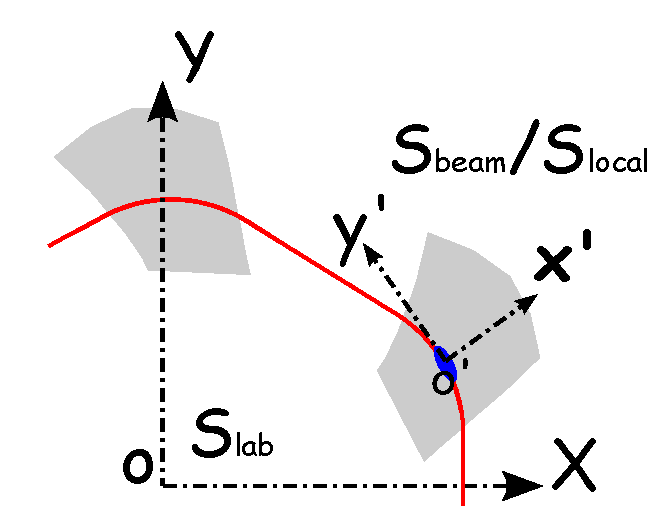
\includegraphics[width=8cm]{figures/SM-frame.pdf}}
    \caption{Schematic plot of the top view of the three coordinates frames. The red curve is the orbit of beam center, 
      the blue area represents beam shape, and the gray area is the hill region of magnetic field.}
    \label{fig:frame}
  \end{figure}

At each time step, to solve space charge fields, the frames $\bs{S}_{\RM{local}}$ and $\bs{S}_{\RM{beam}}$ are redefined according to current 6D 
phase space distribution, and all particles are transformed from $\bs{S}_{\RM{lab}}$ to $\bs{S}_{\RM{local}}$, 
then a Lorentz transformation is performed to transformed all particles to $\bs{S}_{\RM{beam}}$.
After that we can solve the Poisson equation in frame $\bs{S}_{\RM{beam}}$. In a 3D Cartesian frame, the solution of the Poisson equation at point $(x,y,z)$ can be expressed by 
\begin{equation}\label{eq:Poten}
  \phi(x,y,z)= \frac{1}{4\pi\varepsilon_0}\int{G(x,x',y,y',z,z')\rho(x',y',z')dx'dy'dz'},
\end{equation}
where $\rho $ is the charge density function and $G$ is the 3D Green function which can be expressed by Eq.\,(\ref{eq:Green}) under the open boundary conditions.
\begin{equation}\label{eq:Green}
  G(x,x',y,y',z,z')= \frac{1}{\sqrt{(x-x')^2+(y-y')^2+(z-z')^2}}.
\end{equation}
In the following the typical steps of calculating space charge fields using Hockney's FFT algorithm\cite{Hockney:1}(following quantities with superscript $D$ means on grid) are listed.
\begin{itemize}
\item Create 3D rectangular grid domain which contains all particles and doubled it in each dimension, 
\item Assign the charge $q$ of each macro-particle to nearby mesh points to obtain $\rho^D$, 
\item Perform Lorentz transform to obtain $\rho^D$ in beam rest frame $\bs{S}_{\RM{beam}}$,
\item Use FFT on $\rho^D$ and $G^D$ to obtain $\widehat{\rho}^D$ and $\widehat{G}^D$,
\item Determine $\widehat{\phi}^D$ on the grid using $\widehat{\phi}^D = \widehat{\rho}^D \cdot \widehat{G}^D$,
\item Use inverse FFT on $\widehat{\phi }^D$ to obtain $\phi^D$,
\item Compute $\bs{E}^D= -\nabla \phi^D$,
\item Interpolate $\bs{E}$ at the particle positions $\bs{x}$ from $\bs{E}^D$,
\item Perform Lorentz back transform to obtain $\bs{E_{\RM{sc}}}$ and $\bs{B_{\RM{sc}}}$ in  frame $\bs{S}_{\RM{local}}$ and transform back  to $\bs{S}_{\RM{lab}}$.
\end{itemize}

With respect to the external magnetic field, there are two possible situations. 

In the first situation, the real field map is available on the median plane of the existing cyclotron machine using measurement equipment.
In view of the narrow gaps of magnets, in most cases concerning cyclotrons, the vertical field $B_z$ is measured on the median plane ($z=0$) only.
Since the magnetic field outside the median plane is required to compute trajectories with $z \neq 0$, the field needs to be expanded in $Z$ direction. 
According to the approach given by Gordon and Taivassalo\cite{Gordon:2}, by using a magnetic potential and measured $B_z$ on the median plane
at the point $(r,\theta, z)$ in cylindrical polar coordinates, the 3$th$ order field can be written as    
\begin{eqnarray}\label{eq:Bfield}
  B_r(r,\theta, z) & = & z\frac{\partial B_z}{\partial r}-\frac{1}{6}z^3 C_r, \nonumber\\    
  B_\theta(r,\theta, z) & = & \frac{z}{r}\frac{\partial B_z}{\partial \theta}-\frac{1}{6}\frac{z^3}{r} C_{\theta}, \\     
  B_z(r,\theta, z) & = & B_z-\frac{1}{2}z^2 C_z,  \nonumber    
\end{eqnarray}
where $B_z\equiv B_z(r, \theta, 0)$ and  
\begin{eqnarray}\label{eq:Bcoeff}
  C_r & = & \frac{\partial^3B_z}{\partial r^3} + \frac{1}{r}\frac{\partial^2 B_z}{\partial r^2} - \frac{1}{r^2}\frac{\partial B_z}{\partial r} 
        + \frac{1}{r^2}\frac{\partial^3 B_z}{\partial r \partial \theta^2} - 2\frac{1}{r^3}\frac{\partial^2 B_z}{\partial \theta^2}, \nonumber  \\    
  C_{\theta} & = & \frac{1}{r}\frac{\partial^2 B_z}{\partial r \partial \theta} + \frac{\partial^3 B_z}{\partial r^2 \partial \theta}
        + \frac{1}{r^2}\frac{\partial^3 B_z}{\partial \theta^3},  \\
  C_z & = & \frac{1}{r}\frac{\partial B_z}{\partial r} + \frac{\partial^2 B_z}{\partial r^2} + \frac{1}{r^2}\frac{\partial^2 B_z}{\partial \theta^2}. \nonumber
\end{eqnarray}

All the partial differential coefficients are computed on the median plane by interpolation. This code uses Lagrange's 5-point formula.

In the other situation, 3D fields for interesting region are calculated numerically by building a 3D model using commercial software 
during the design phase of a new cyclotron . In this case the calculated field will be be more accurate, especially at large distances from the median plane.

Finally both the external fields and space charge fields are used to track particles for one time step using a 4$th$ order Runge-Kutta (RK) integrator, in which 
the fields are evaluated for four times in each tracking step. Space charge fields are assumed to be constant during one tracking step,
because their variation is typically much slower than that of external fields. 
    
\section{NEIGHBORING BUNCH EFFECTS}
%1. self-consistent model using multi-bunch track strategy, advantage and disadvantage. 
%2. energy bin and rebin trick in cyclotron.
%3. new bunch injection trick. 
In cyclotrons the turn separation $\Delta R$ is affected by many factors. They include the machine characteristics such as magnetic field map, 
voltage profile and the accelerating phase of the RF resonators. In addition the initial centering conditions of the injected bunches have to be considered. 
The typical tendency is that  $\Delta R$ reduces gradually  with increasing beam energy.
For some machines, $\Delta R$ stays sufficiently large from injection to extraction, and in such cases,  neighboring bunch effects are negligible. 
For others, $\Delta R$ decreases strongly during the course of acceleration resulting in the need to consider neighboring bunch effects in order to
obtain a correct description of the physical behavior.

In our model, initially one bunch with $N_p$ particles is injected at the average radial position $R_0$ (is stored) and tracked for one turn. 
After exactly one revolution period $T_{r}$ the new radial position $R_1$ is recorded again. If the condition
\begin{equation}\label{eq:dR}
  \Delta R \equiv R_1-R_0 \le M \times r_{\RM{rms}},
\end{equation}
is fulfilled, where $r_{\RM{rms}}=\sqrt{x_{\RM{rms}}^{2}+y_{\RM{rms}}^2}$ and $M$ are parameters given by the user, the 6D phase space data $(x, p_x, y, p_y, z, p_z)$ at this time step is stored. 
After it is further tracked for another $T_{r}$, the code is switched to multi-bunch mode. 
A new bunch is injected by reading the 6D phase space data stored before and the two bunches are tracked simultaneously.
The third bunch is then injected in the same way after another turn, and so forth, until the maximum bunch number $N_B$ is achieved in the simulation. $N_B$ is also set by the user.
The underlying assumption for this is that all bunches have the same phase space distribution when they reach a certain position.
This is realistic and reasonable when the machine is running in a steady state.  

To the contrary, if the condition of Eq.\,(\ref{eq:dR}) is not fulfilled,
%\begin{equation}\label{eq:dR1}
%  \Delta R \equiv R_1-R_0  > M \times r_{rms},
%\end{equation}
the code continues to track a single bunch until Eq.\,(\ref{eq:dR}) is valid.   

Here another question raises. How many bunches should be simulated to evaluate neighboring bunch effects? 
  
\begin{figure}
    {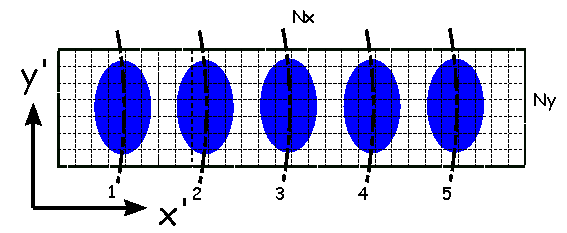
\includegraphics[width=8cm]{figures/SM-MultiBunch.pdf}}
    \caption{Schematic plot of the top view of 5 bunches and the grid of computation domain. The grid size on $X'-Y'$ plane is Nx$\times$Ny, and the broken lines represent the orbits of beam centers. }
    \label{fig:MultiBunch}
\end{figure}

In order to answer this question, let's first do a physical analysis for the case of 5 bunches, as shown schematically in Fig.\,\ref{fig:MultiBunch}.
Here the objective of study is the evolution of the center bunch, namely bunch 3. 
Neighboring bunch effects are eventually derived from all the interactions of individual particles in the bunches. 
The electric field between two point charge is proportional to $1/r^2$, where $r$ is their distance. In this case, for bunch 3, the sources
of neighboring bunch effects mainly come from the direct space charge force of bunch 2 and 4 (of the first order), which are much stronger than those from bunch 1 and 
5 (of the second order). However, bunch 1 and 5 also have indirect impacts on bunch 3, 
namely by their direct space charge force (of the first order) to the evolution of bunch 2 and 4, respectively. 

In order to obtain a more accurate and consistent solution, one needs to employ more bunches. In theory, when the maximum bunch number $N_B$ equals the total turn number of the machine, one can eventually obtain the fully self-consistent solution of the problem by our model. 
In reality, it is impossible to simulate a full set of bunches which typically range from 
several ten to several hundred.
The scale of particle number and the dimensions of the grid are beyond the capability of today's computer resources.

A pragmatic approach is given by doing the simulation for 3 bunches and 5 bunches and comparing phase space results first. If the discrepancy is visible, one needs to do 
the simulation for 7 bunches, and compare its result with 5 bunches, and so forth. 
Eventually, with the proper setting of $N_B$ and $M$, neighboring bunch effects can be evaluated precisely.
For instance, the setting with $N_B=9, M=4.5$ gives a precise result for the PSI Ring cyclotron of 3\,mA beam current.
We will discuss this in more detail in the following section. 

In a multi-bunch simulation the energy of bunches in different turns is quite different. One can't find a single beam rest frame in which the relative motions of 
particles are non-relativistic. Consequently it is not sufficient to use only one rest frame 
and a single Lorentz transformation. In order to calculate space charge fields more precisely, we introduce an adaptive binning technique.
First we calculate the average $\bar{\gamma_i}$ for th $i$th bunch with $N_p^i$ simulation particles
\begin{equation}\label{eq:dR1}
  \bar{\gamma}_i = \frac{\sum_{j=1}^{N_p^i}\sqrt{1+p_{j,x}^2+p_{j,y}^2+p_{j,z}^2}}{N_p^i}.
\end{equation}
Then every particle is grouped into the energy bin whose $\bar{\gamma_i}$ is closest to its $\gamma$. In this way, the energy spread of each bin is relatively small and relative motions of the particles in the same bin are non-relativistic.
After binning we perform the Lorentz transformation, calculate the space charge field and perform back-transformation for each bin respectively. 
Finally the field data is summed up to give out the total space charge force imposed on each particle.

The energy spread of bunches can be quite large, especially in cyclotrons without flat-top cavities, and at large radii. This may result in an overlap of 
energy distributions of bunches in neighbored turns. In this case, the energy bins have to be recalculated and all particles are regrouped frequently.

It is worth noting that, in cyclotrons, the energy gain per turn is varying as a function of radius. 
So $\Delta\bar{\gamma}_i= \bar{\gamma}_i-\bar{\gamma}_{i-1}$ is not a constant parameter, either. Therefore, one should not set $\Delta\bar{\gamma_i}$ of the bins 
the same interval, as done in some codes to deal with large energy spread of single bunch in LINAC and photoinjector.

\section{IMPLEMENTATION UNDER \opal \  FRAMEWORK}
%1. Brief introduction of OPAL characteristic.
%2. The Hierarchical layout of code.
%3. Introduction of functionality of OPAL-cycl.

Above model and algorithm are implemented in the object-oriented parallel PIC code \opalcycl. 
\opalcycl \  is one of the flavors of the \opal \ (Object Oriented Parallel Accelerator Library) framework \cite{opal:1}, a generic library
initialized by A. Adelmann. This framework is a powerful tool for charged-particle optics in general accelerator structures and beam lines.
Using the MAD languages with extensions,
\opal \  is derived from MAD9P \cite{Ada:1} and is based on the CLASSIC \cite{Classic:1} library and IPPL framework(cite?). 
CLASSIC library is a C++ class library which provides services for building portable accelerator models and algorithms and input 
language to specify complicated accelerator systems in general. IPPL is a Object-Oriented C++ class library which provides a flexible
environment for data-parallel programming of scientific application. It provides an integrated, layered system of objects. The upper layers
contain global data objects of physical/mathematical quantities, such as particles, fields and matrices of meshes and typical methods
performed on these objects such as binary operators and FFT. the lower layers contain the object's relevant to parallelization and efficient node-level
simulation, such as data distribution, domain decomposition and communication among processors, load balancing and chained-expression optimization. 
The intermediate phase space data of all particles and some interesting parameters, 
including RMS envelop size, RMS emittance, energy, path length, bunch numbers and 
tracking step, are stored in the H5Part\cite{H5part:1} file-format and can be analyzed
using the visualization tool H5PartRoot(\url{http://amas.web.psi.ch/tools/H5PartROOT/index.html}).

In addition, apart from the multi-particle simulation mode, \opalcycl \  also has two other serial tracking modes for conventional cyclotron machine design. 
One mode is the single particle tracking mode, which is a useful tool for 
the preliminary design of a new cyclotron. It allows to compute  basic parameters, such as reference orbit, phase shift history,
stable region and matching phase ellipse. The other one is the tune calculation mode, which can be used to compute the betatron oscillation frequency 
$\nu_r$ and $\nu_z$. This is useful for evaluating 
the focusing characteristics of a given magnetic field map. 

A more detailed description of the hierarchical layout, the parallelization and the implementation issues of the \opal \  framework and \opalcycl \  code
can be found in the User's Reference Guide \cite{opal:1}.  


\section{PERFORMANCE TEST AND VALIDATION}
In order to evaluate the performance and benchmark the functionalities of the newly developed code, we performed different types of simulations on
 the 72\,MeV Injector\,II cyclotron of PSI, which has been studied intensively before. Some results are presented in this section. 

\subsection{Single particle tracking and tune calculation}
In theory, there is an eigen-ellipse for any given energy in a cyclotron under stable conditions. Only when the initial phase space
matches this eigen-ellipse, the oscillation of the beam envelope amplitude will be minimal and the transmission efficiency will be maximal.
In this test, the eigen-ellipse at 2\,MeV kinetic energy was calculated using the single particle tracking mode of \opalcycl \ ,    
and the result was compared with the result given by FIXPO\cite{FIXPO:1}, which is the standard orbit integration program of PSI.
Fig.\,\ref{fig:Eigen} shows the matched radial ellipse with an initial offset of $\Delta r=2.0{\RM{\,mm}}$, $\Delta p_r=0.0{\RM{\,mrad}}$ at symmetry line of the sector field. 
A perfect agreement is obtained when the time step is set to 1\,ps in\opalcycl, although FIXPO uses a different tracking algorithm with the azimuthal angle as
the independent variable.
\begin{figure}
  {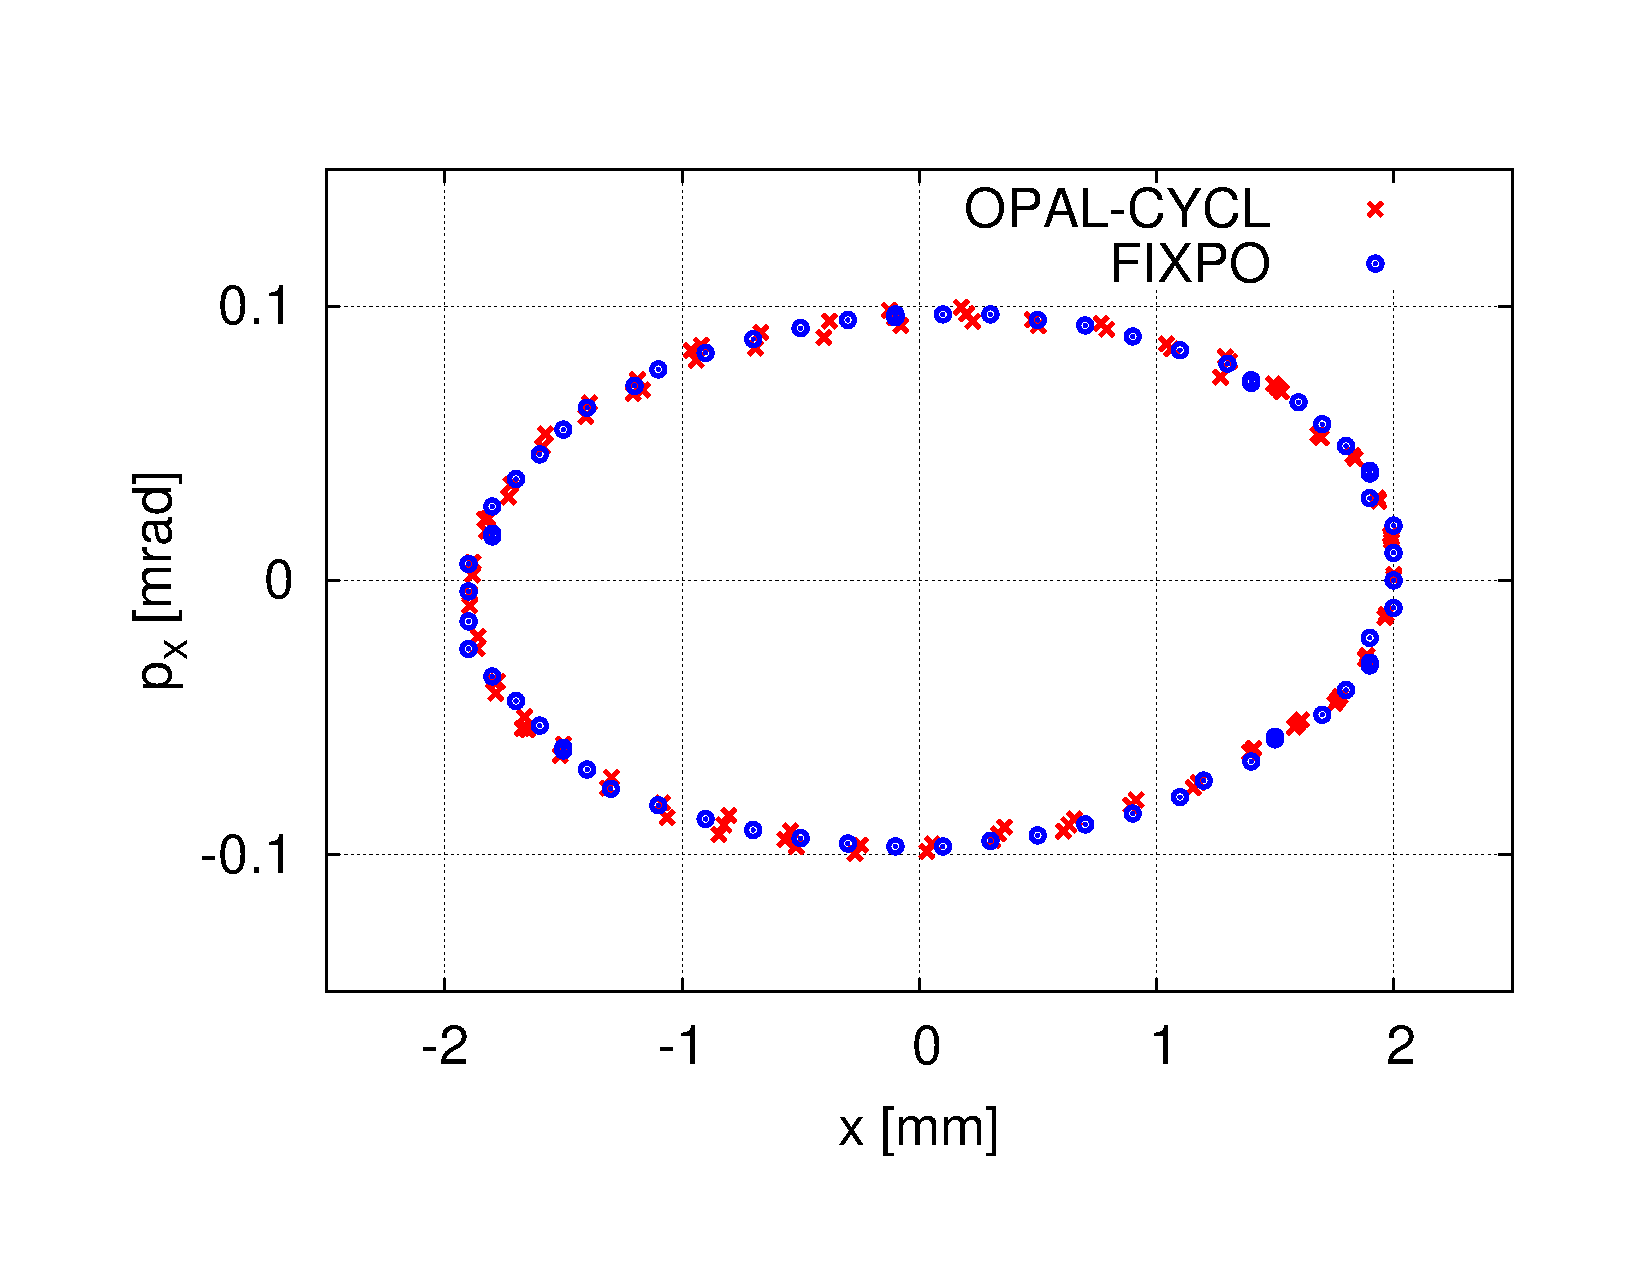
\includegraphics[width=8cm,trim=2.5cm 2.5cm 2.5cm 2.5cm]{figures/RadialEigen_Inj2.pdf}}
  \caption{Radial eigen ellipse of 2\,MeV at the symmetric line of magnet in Injector\,II cyclotron.}
  \label{fig:Eigen}
\end{figure}

The tuning digram of Injector\,II was computed using the tune calculation mode of \opalcycl, as shown in Fig.\,\ref{fig:nurnuz_Inj2}.
The result from FIXPO and \opalcycl \ agree very well, although they use different numerical algorithms to calculate the tune. 
\begin{figure}
  {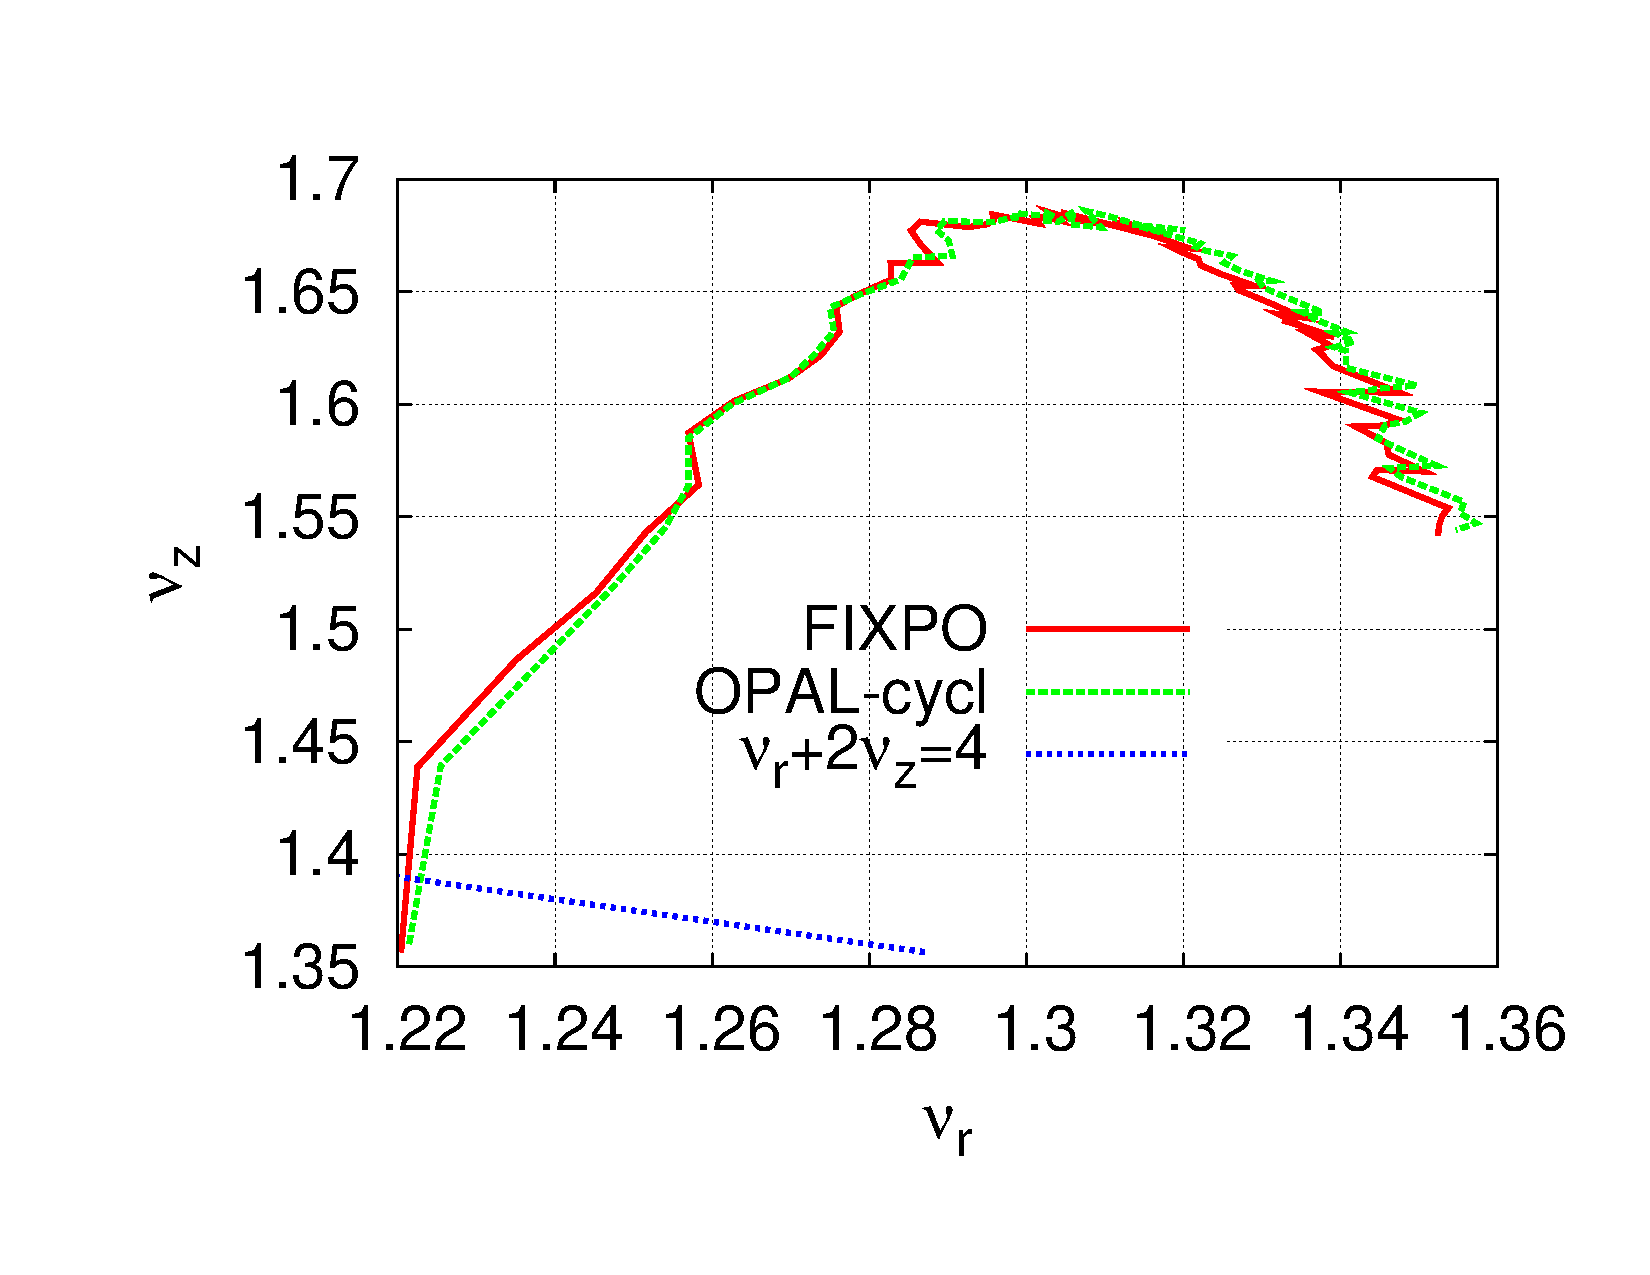
\includegraphics[width=8cm,trim=2.5cm 2.5cm 2.5cm 2.5cm]{figures/nurnuz_Inj2.pdf}}
  \caption{Tune diagram of Injector\,II cyclotron, compared with FIXPO code.}
  \label{fig:nurnuz_Inj2}
\end{figure}

The field interpolation scheme, particle tracking and tuning calculation functionalities are validated substantially by the above tests. 
\subsection{Parallel scalability test}
In order to observe the parallel scalability of the code, we have performed a detailed comparison of time consumption using different number of processors. 
In this test, 1\,million particles are used in total to track 200 time steps on Injector\,II. The initial beam has a Gaussian
type distribution. The grid size is $64 \times 64 \times 64$ which is decomposed onto a two dimensional grid of processors. All the intermediate phase space data is dumped into 
a single H5Part file. The dynamic load balancing frequency as well as the phase space dumping frequency are set to 10.
The results are shown in Fig.\,\ref{scalability}.
\begin{figure}
  {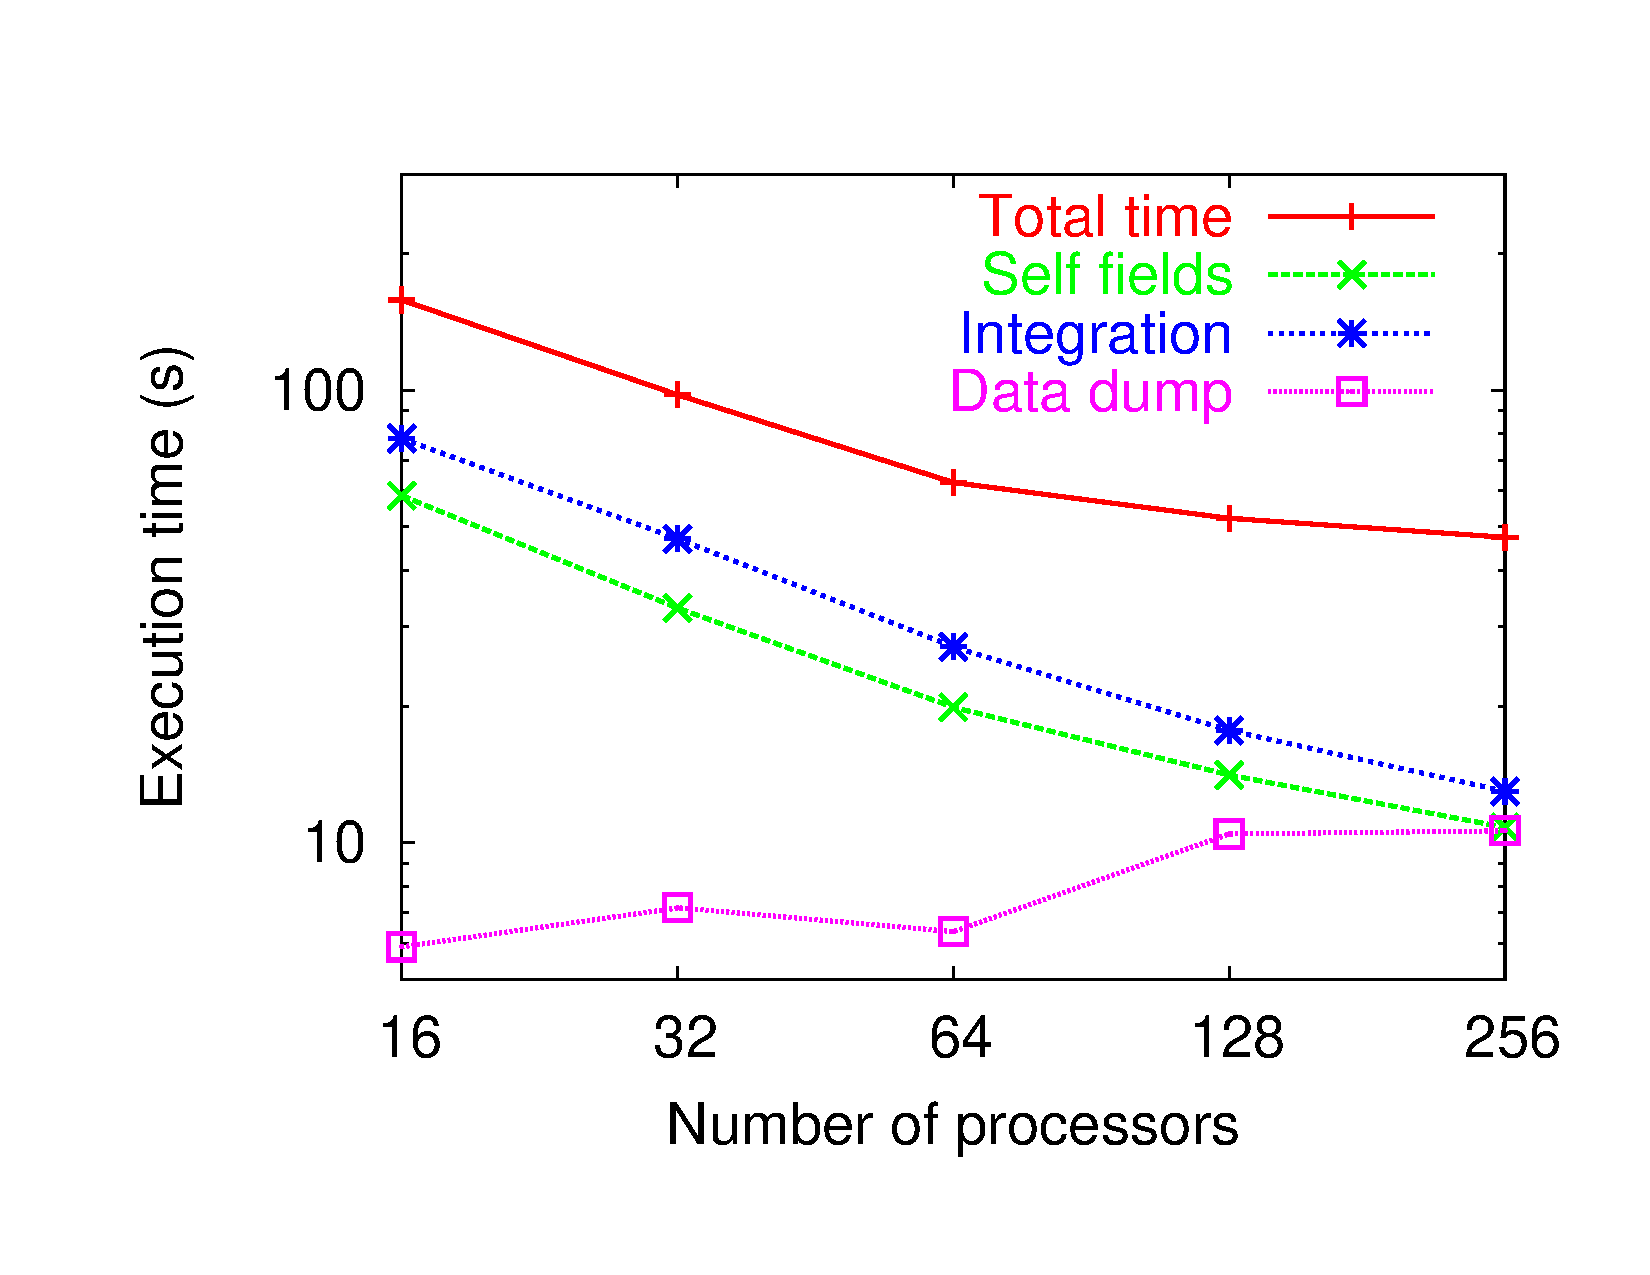
\includegraphics[width=8cm,trim=0cm 0cm 0cm 0cm]{figures/Timing64mesh.pdf}}
  \caption{The time consumption as a function of processors on Cray XT3, CSCS.}
  \label{scalability}
\end{figure}

We can see that a good scalability is achieved up to 128 processors. When the number of processors reaches 128, the time consumption of the phase space dumping starts to become significant for the total computation time.
The reason is that the data is dumped into a single file and the data exchange between root node and other nodes increases significantly.
Nevertheless, the scalability of the space charge solver and the particles integrator still benefit from a large number of processors.
\subsection{Stable compact beam in Injector\,II}
Space charge effects usually can result in the increase of beam size and emittance, so it is usually harmful for the beam dynamics. 
But in some cases, space charge effects can play a positive role. PSI Injector\,II cyclotron is a space charge dominated machine, in which a very compact 
stable beam is developed within the first several turns, and thereafter, this charge distribution with extremely narrow phase width (about $2^o$) 
remains essentially unchanged until extraction. This is the combined effects of the strong coupling between 
radial and longitudinal direction in cyclotron and space charge when the beam current increases above 1\,mA. S. Adam first reproduced this phenomenon by 
using a serial two-dimensional code PICN \cite{Adam:1}. PICN is based on the Needle model, which treats the beam as 
an ensemble of changed vertical needles with the same height as the beam. In this model, the vertical motion of particles is separated form the horizontal 
one and the internal motion within needles is neglected. In order to validate the space charge solver module of our code, we performed the 1\,mA, 3\,MeV coasting beam simulation on this machine and compared the result with PICN.  

We used the same initial distribution as in ref.\cite{Adam:3}.
$2\sigma_{\RM{longitudinal}} = 13.4 {\RM{\,mm}}$ ( $15^o$ phase width), $2\sigma_{\RM{transverse}} = 2.52 {\RM{\,mm}}$. 
The initial emittances of the radial and azimuthal direction are set to zero. 
In the vertical direction, $2\sigma_z = 4{\RM{\,mm}}$, $2\sigma_{p_z} = 3.68{\RM{\,mrad}}$. 
The total macro-particles number is 1\,million.  Fig.\,\ref{fig:coasting1mAA} shows the top view of beam shape in the local beam frame.
We can see that a stable core is developed after about 10 turns, which is faster than the formation of stable haloes.

When comparing Fig.\,\ref{fig:coasting1mAA} with Fig.\,3 and Fig.\,4 in ref.\cite{Adam:3} calculated by PICN, we can find the results agree with each 
other qualitative.Both of these two codes predict the formation of a compact stable core and  wide haloes after 40 turns.
However, there exists visible differences. PICN gives out a perfect ``round'' charge density distribution of core and \opalcycl\ gives out a not so perfect round one, namely, the longitudinal size of the core is about 2\,mm longer than the transverse size. The difference should mainly come from the different physics models used in the two codes.
In PICN all those particles close to each other in horizontal plane are represented by a single ``needle'', meanwhile, in \opalcycl\  only those particles close to each other in 6D phase space are represented by a single macro-particle, which is believed to be more realistic and accurate. 

\begin{figure*}
    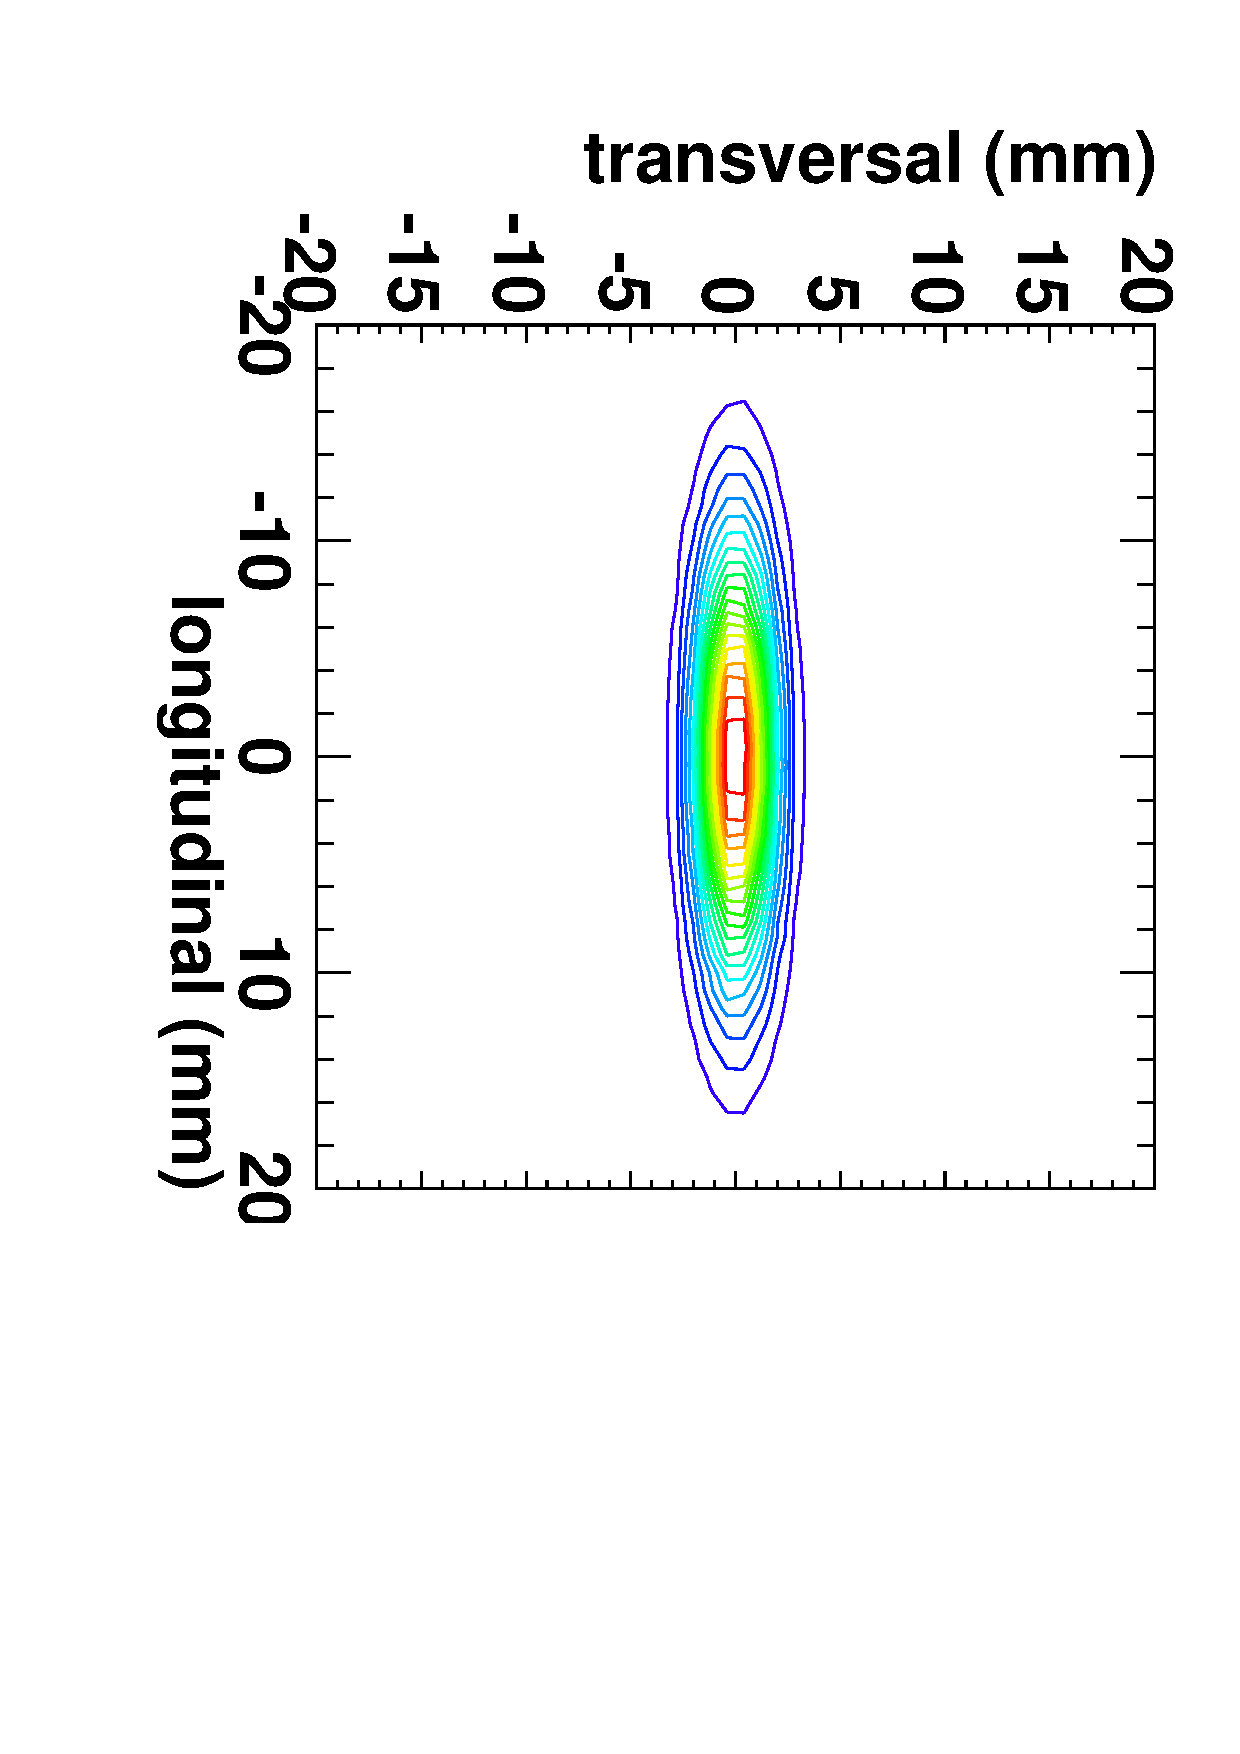
\includegraphics[angle=90,width=0.3\linewidth]{figures/Inj2/1mA0.pdf}
    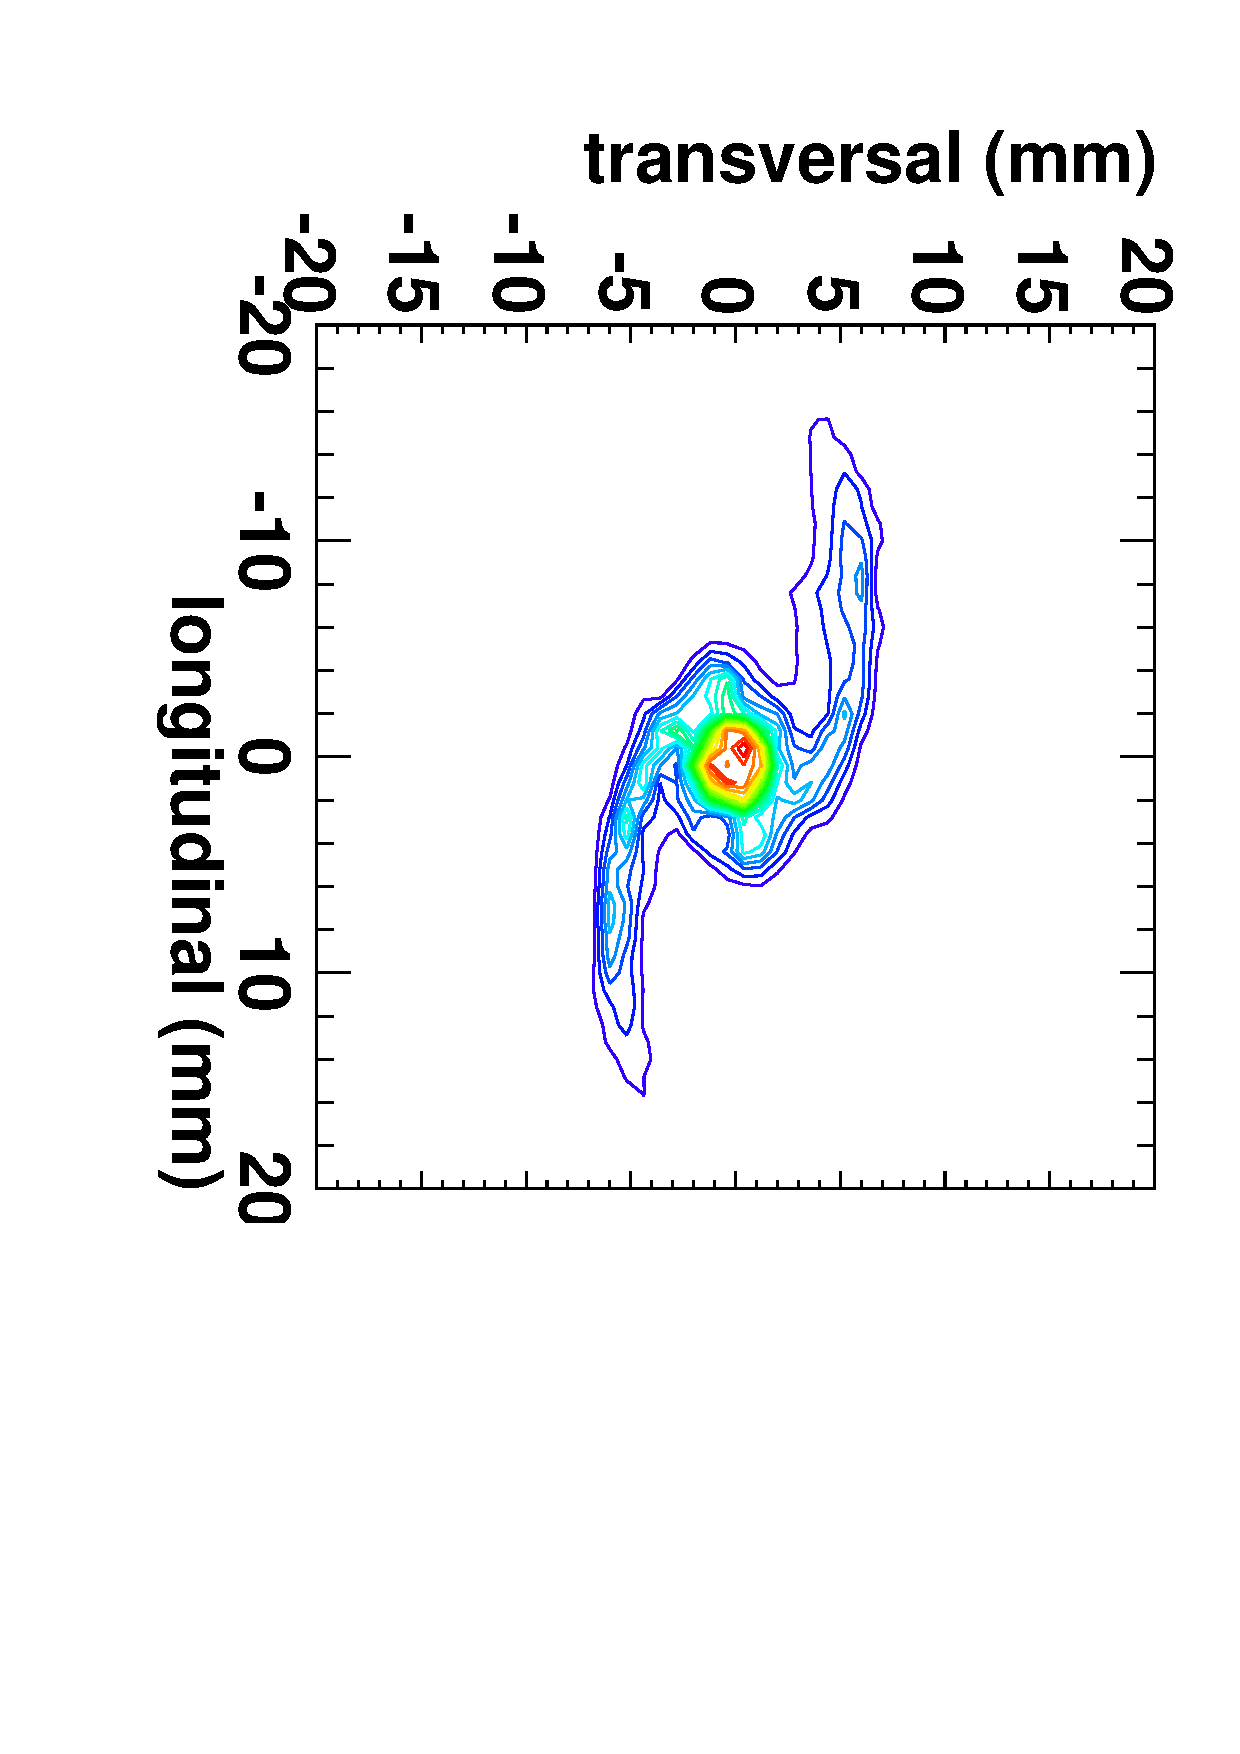
\includegraphics[angle=90,width=0.3\linewidth]{figures/Inj2/1mA5.pdf}
    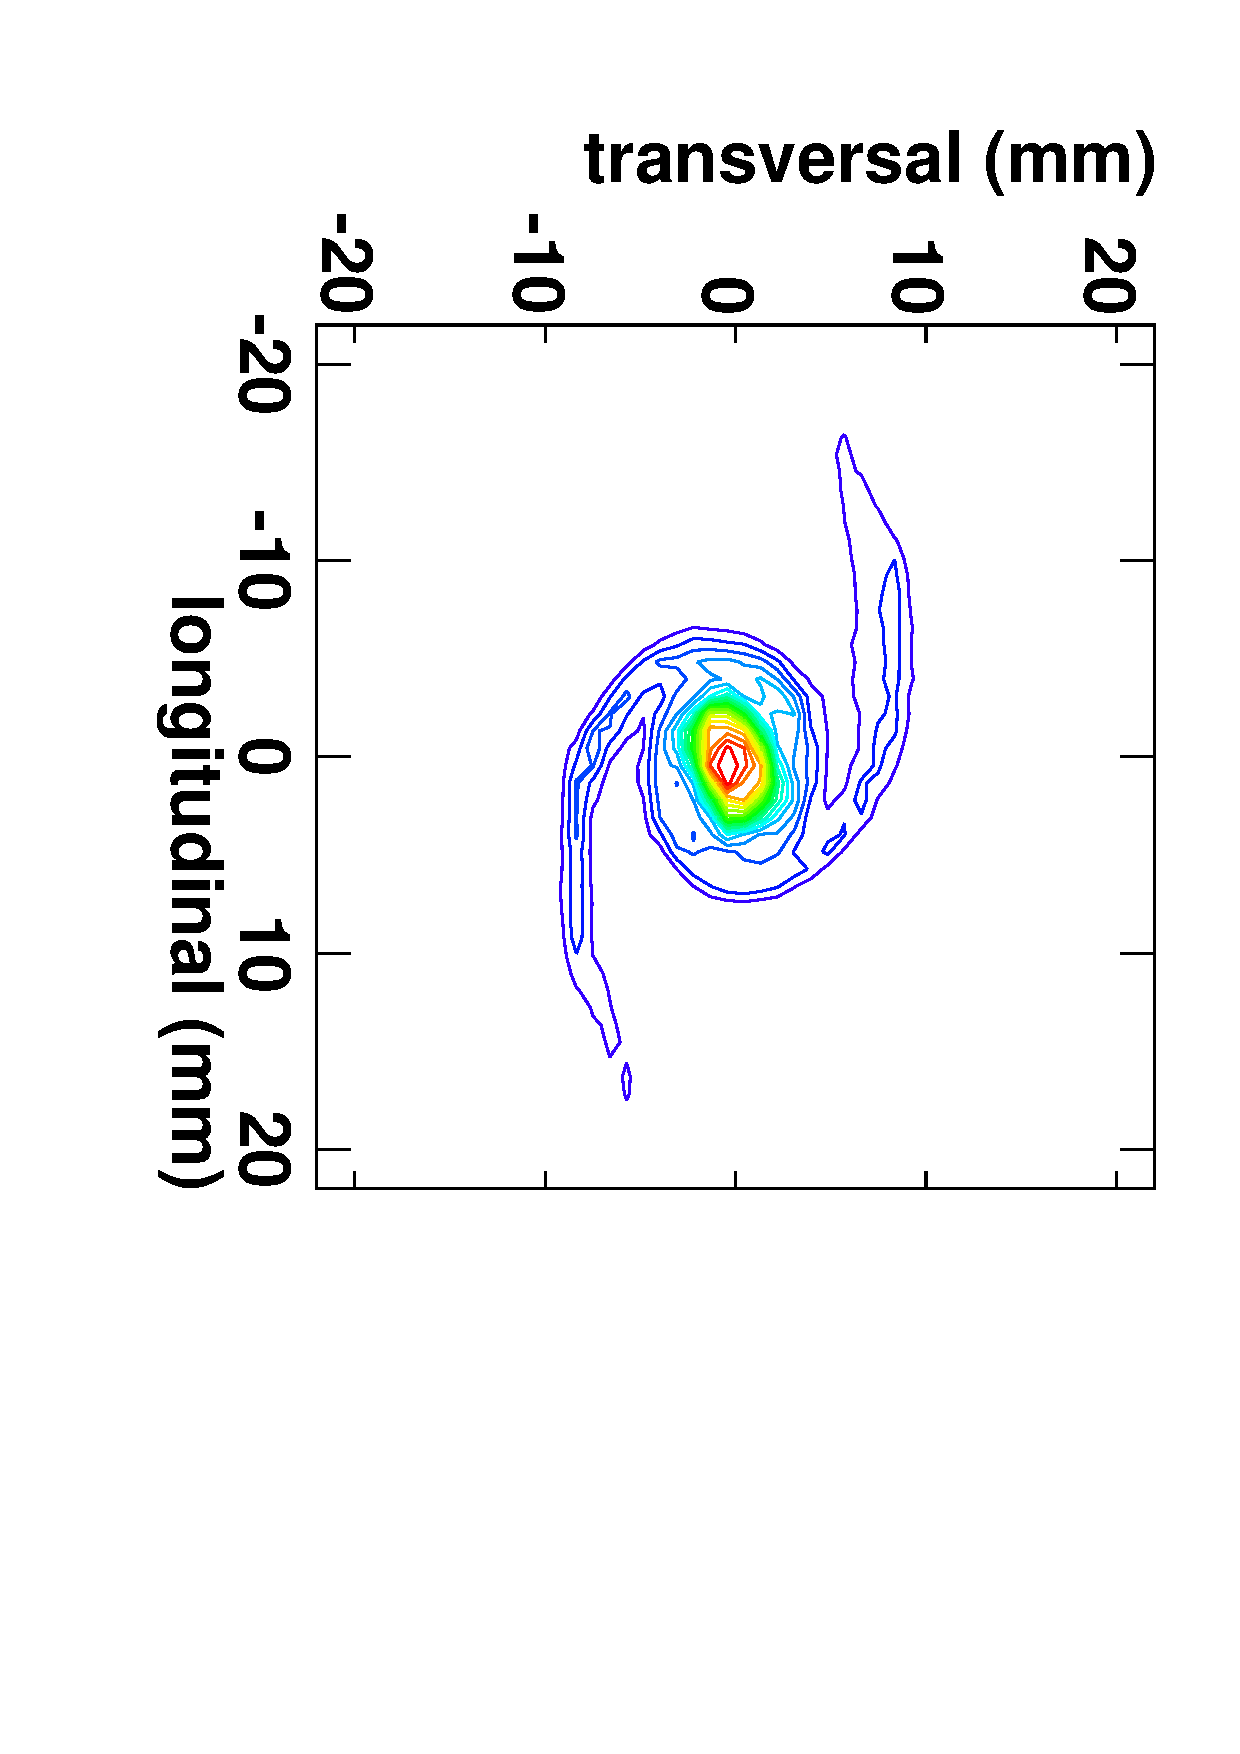
\includegraphics[angle=90,width=0.3\linewidth]{figures/Inj2/1mA10.pdf}
    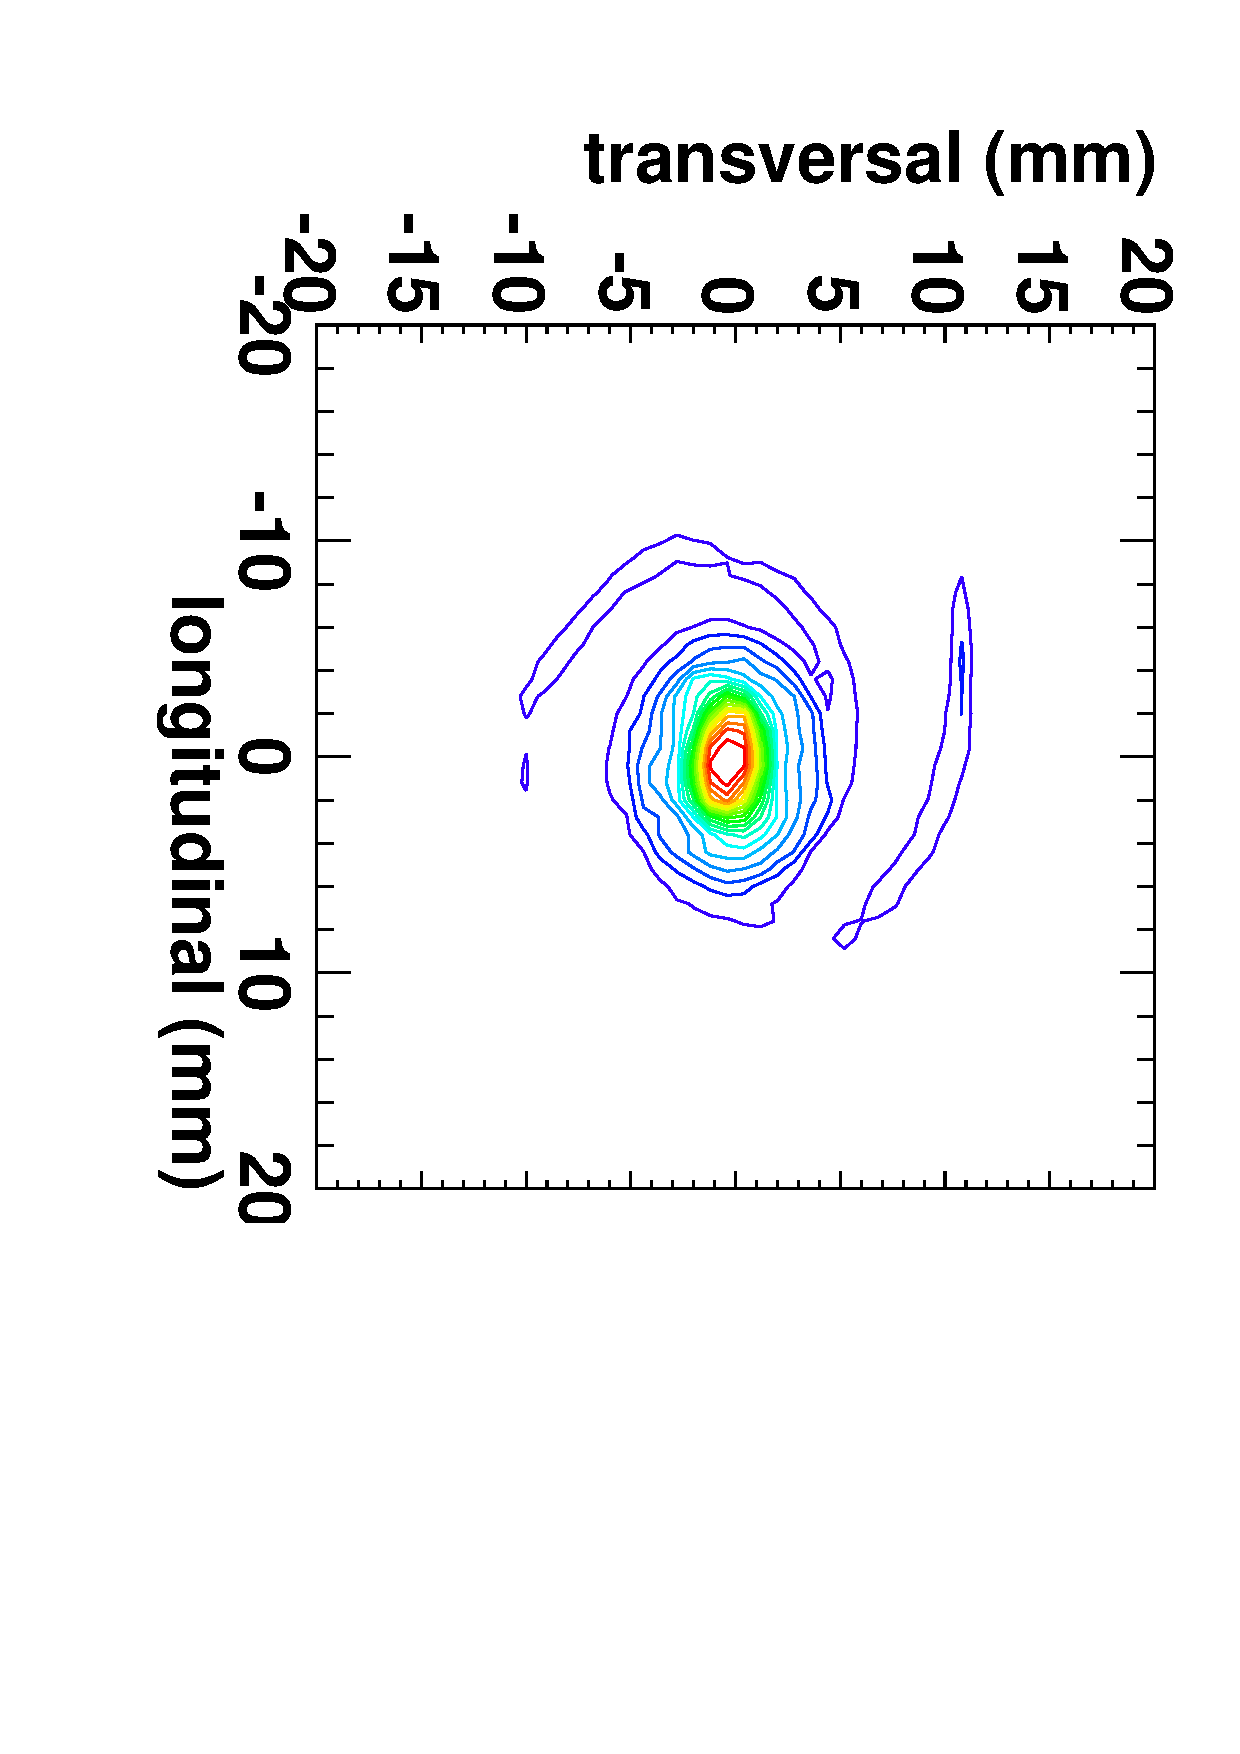
\includegraphics[angle=90,width=0.3\linewidth]{figures/Inj2/1mA20.pdf}
    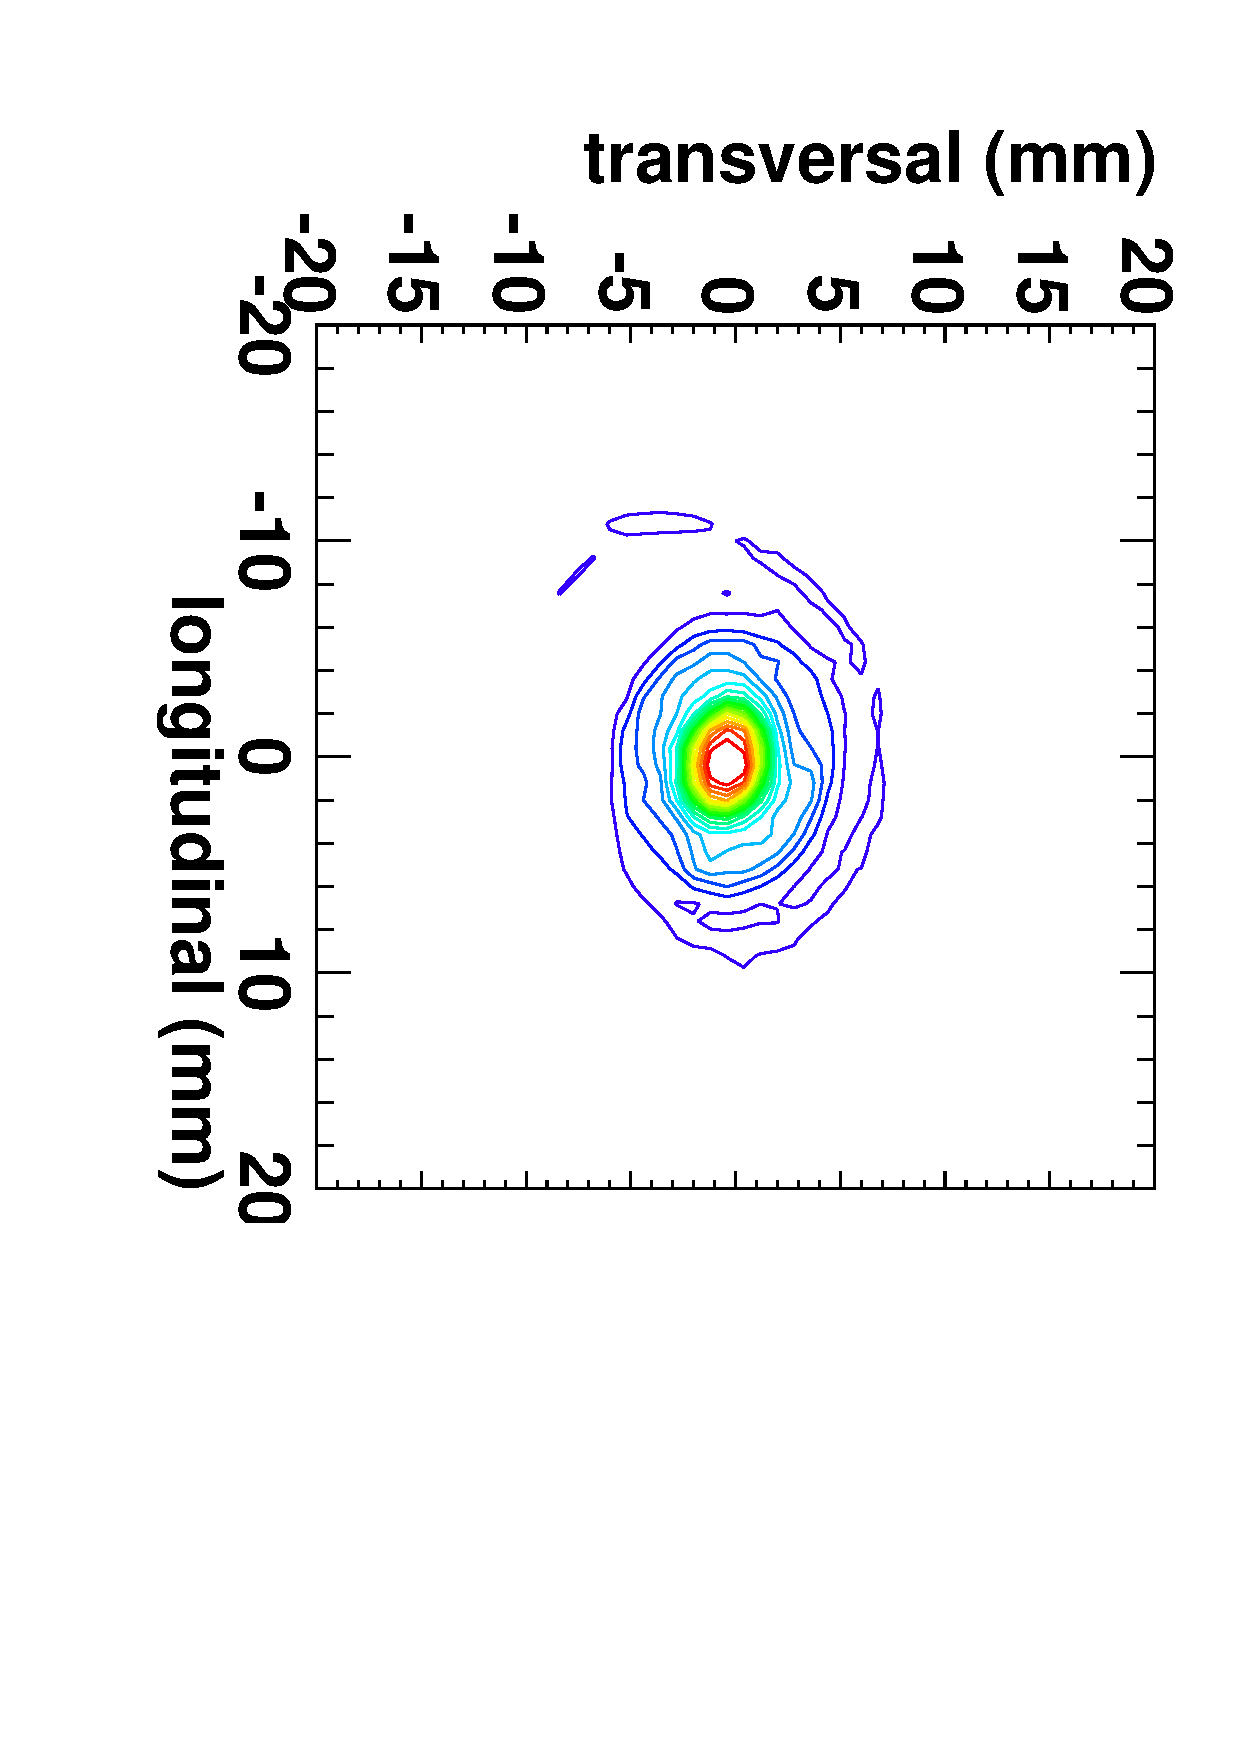
\includegraphics[angle=90,width=0.3\linewidth]{figures/Inj2/1mA30.pdf}
    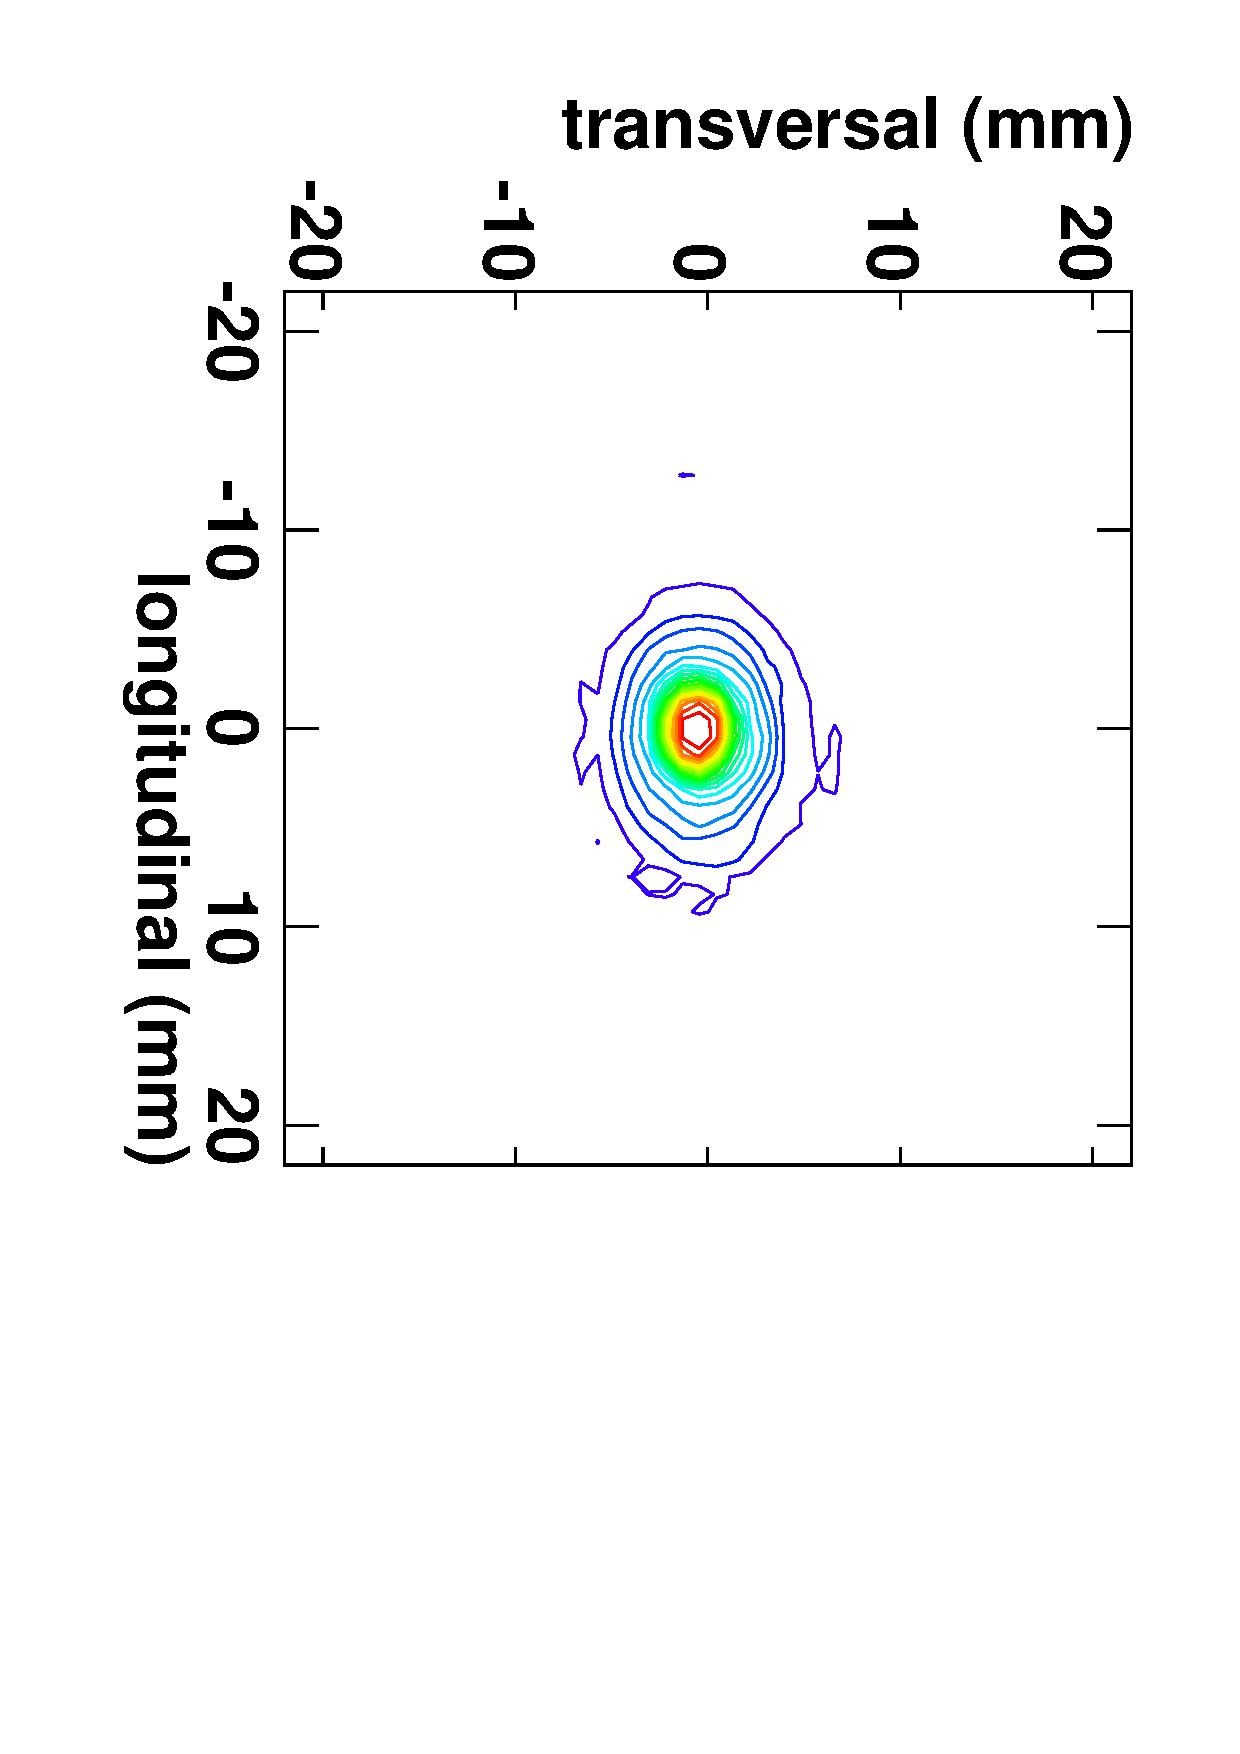
\includegraphics[angle=90,width=0.3\linewidth]{figures/Inj2/1mA40.pdf}
    \caption{Top view of a 1\,mA, 3\,MeV coasting beam in PSI Injector\,II in the local frame ${\bs{S}_{\RM{local}}}$ of PSI Injector\,II. 
      Up: turn 0, 5, 10. Down: turn 20, 30, 40. In order to be comparable with the figure in ref. \cite{Adam:3}, particles are set to propagate left 
      in these plots.}
    \label{fig:coasting1mAA}
\end{figure*}
\section{APPLICATIONS}

\subsection{Different phase widths study of PSI Ring}

Although a very compact beam of about $2^o$ phase widths can be extracted from the Injector\,II, it expands in the longitudinal direction on the 72\,MeV 
beam line because of the space charge effects and chromatic dispersion. For the future 3\,mA beam, this will bring big pressure on the Ring cyclotron.
A super buncher of 10$th$ harmonic is planed to be installed on the beam line to make bunch as short as possible at the injection point of the Ring.
Therefore, how short the bunch should be achieved at the injection point of the Ring is a critical question. 

In order to obtain a clear perspective on this issue, \opalcycl \  was applied to do numerical simulation on the Ring  by tracking Gaussian type beams with 3
different initial conditions. The initial longitudinal phase widths (6$\sigma$) are set to $2^o$, $6^o$ and $10^o$, respectively,
and the initial energy spread is neglected.
The initial conditions on the horizontal and vertical directions are the same. 
%On the horizontal direction, the beam sizes are $12$\,mm and momenta are set to zero. On the vertical direction, beam sizes and momenta are $12$\,mm and $3.4\times10^{-4}$. 
The initial distribution is not correlated in phase space.
The simulation used $10^5$ macro-particles and 32$\times$32$\times$32 gird sizes. The peak voltage of the main resonator and the 3rd harmonic flat-top resonator are 0.9\,MV and
0.403\,MV (11.2\% of accelerating voltage), respectively. The time step is set to 0.1 ns. It takes about 7 hours on CRAY XT3 of CSCS using 64 processors to track particles from the 
injection to the extraction.

\begin{figure*}
  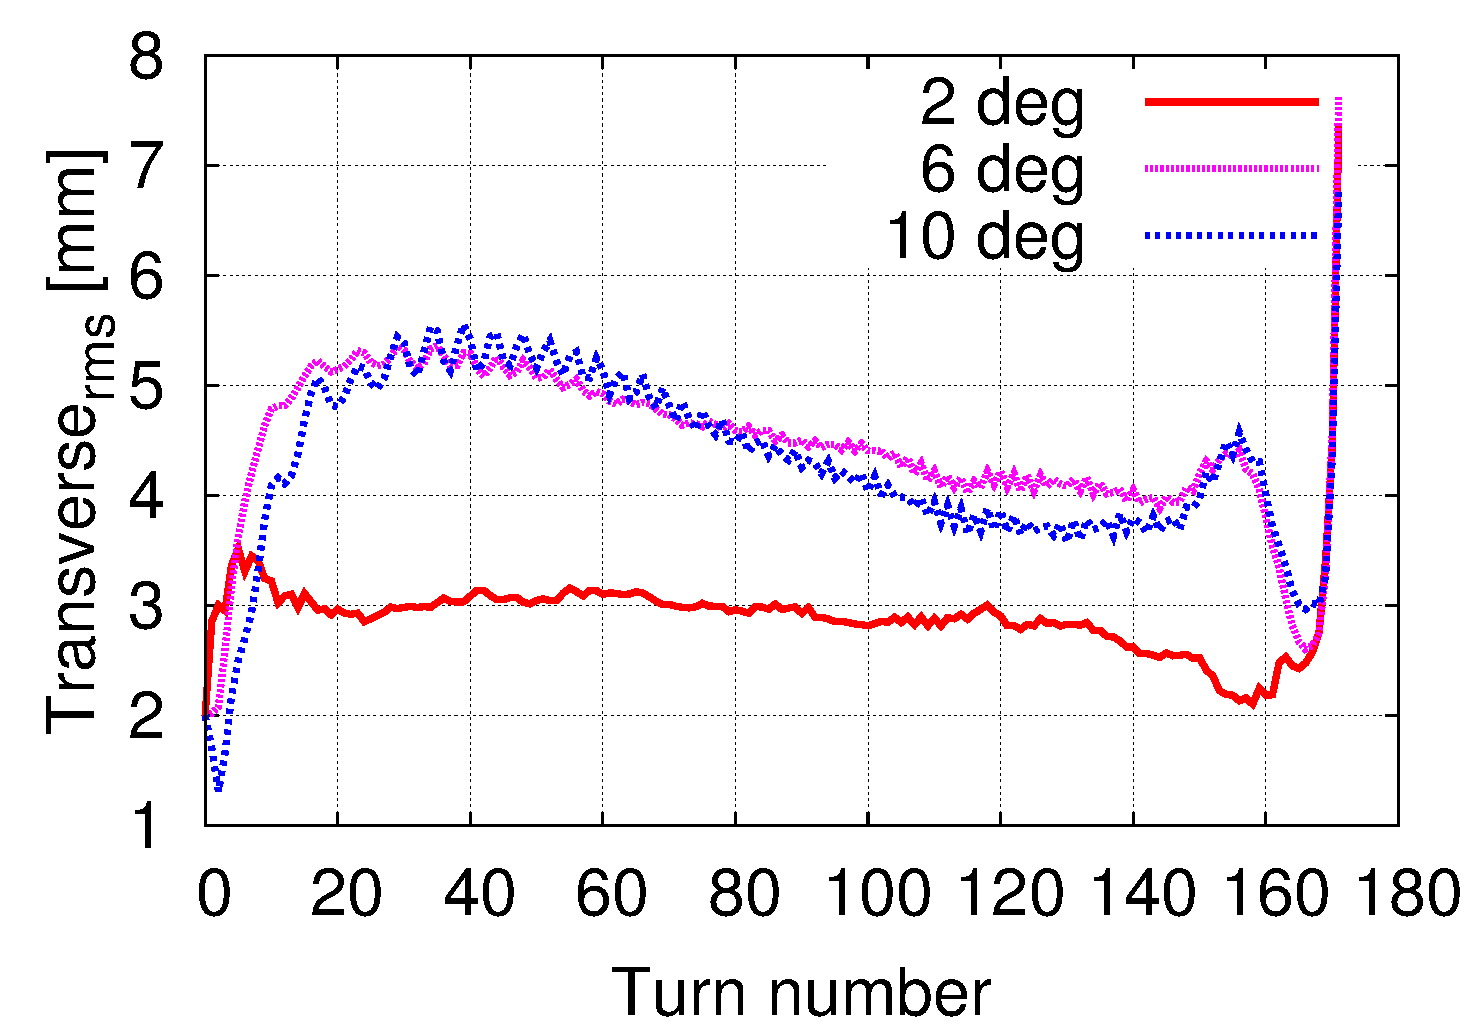
\includegraphics[width=0.45\linewidth]{figures/Comp-Transverse.pdf}
  \includegraphics[width=0.45\linewidth]{figures/Comp-Longitudinal.pdf}
  \caption{Comparison of the rms beam size in the transverse direction (left) and longitudinal direction (right) at $112^o$ azimuthal position of each turn 
    in PSI Ring cyclotron. }
  \label{fig:RMSsize}
\end{figure*}

\begin{figure*}
  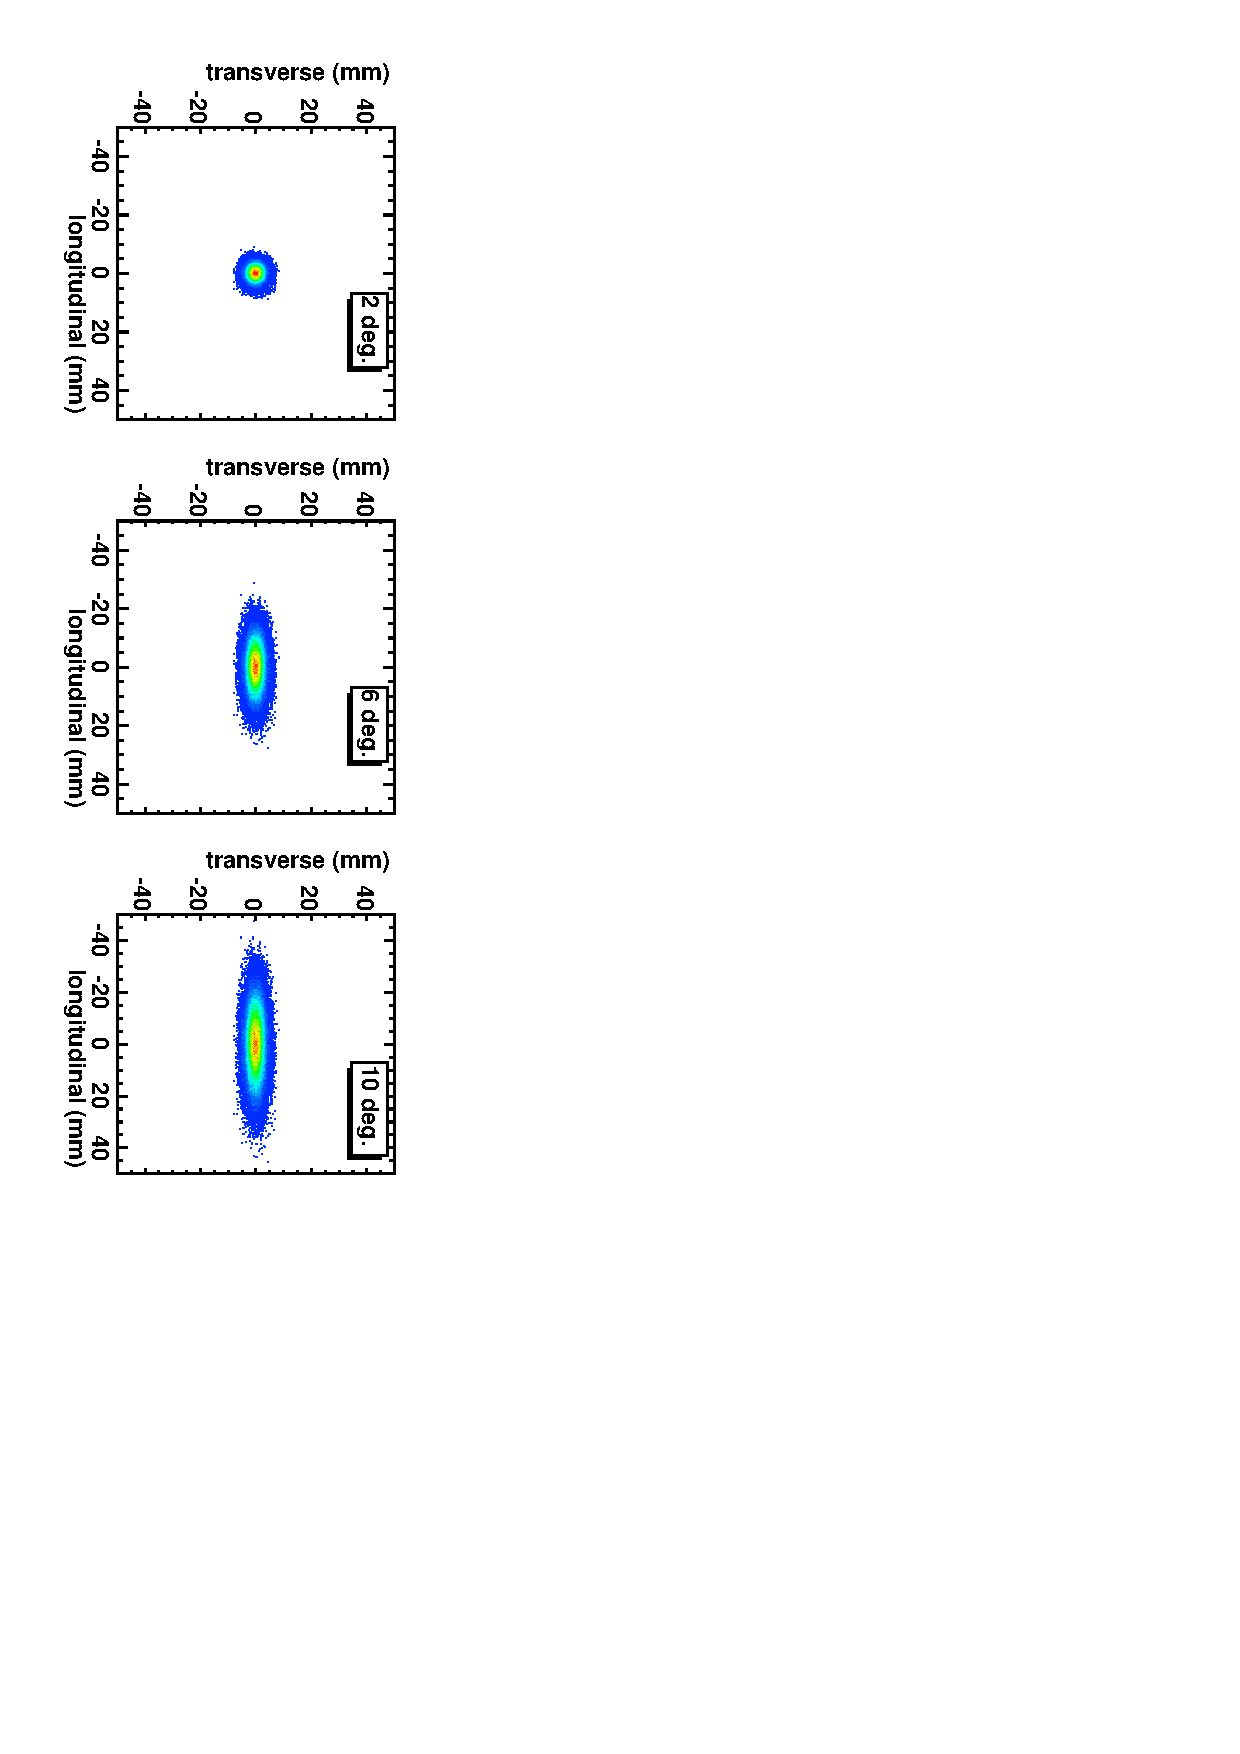
\includegraphics[angle=90,width=0.9\linewidth]{figures/Turn-0.pdf}
  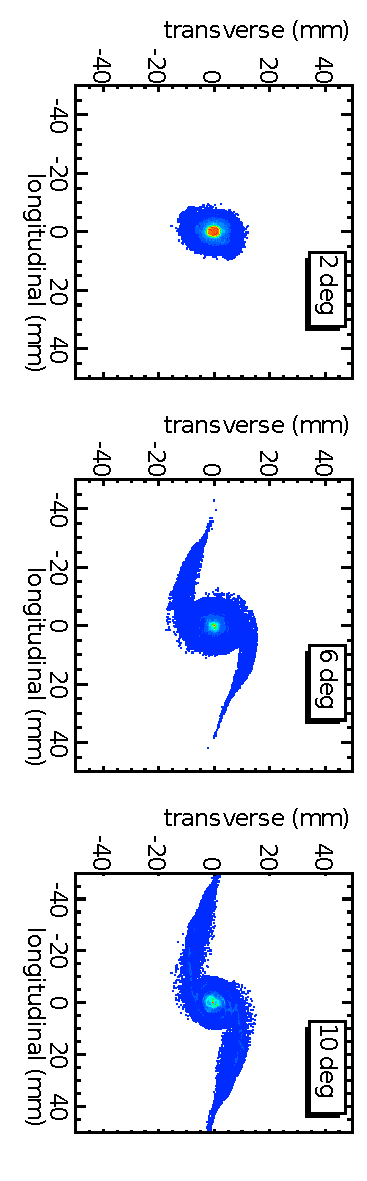
\includegraphics[angle=90,width=0.9\linewidth]{figures/Turn-50.pdf}
  \includegraphics[angle=90,width=0.9\linewidth]{figures/Turn-150.pdf}
  \caption{Top view of 3\,mA bunch distributions with  $2^o$, $6^o$ and $10^o$ initial phase widths at initial position(top) turn 50(middle) and 150(bottom) 
    in the local frame ${\bs{S}_{local}}$ of $112^o$ azimuthal position of PSI Ring cyclotron. }
  \label{fig:RingPhaseWidth}
\end{figure*}

\begin{figure*}
  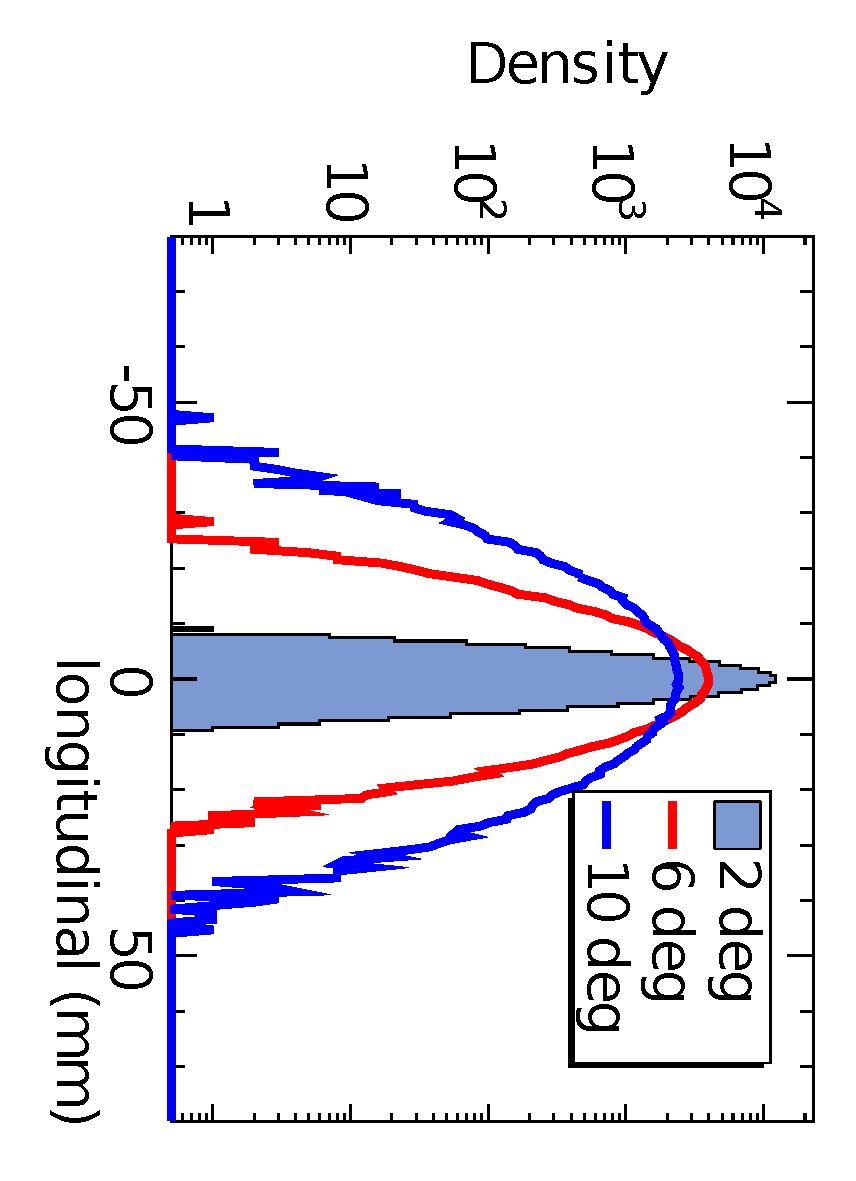
\includegraphics[angle=90,width=0.3\linewidth]{figures/Theta-Turn-0.pdf}
  \includegraphics[angle=90,width=0.3\linewidth]{figures/Theta-Turn-50.pdf}
  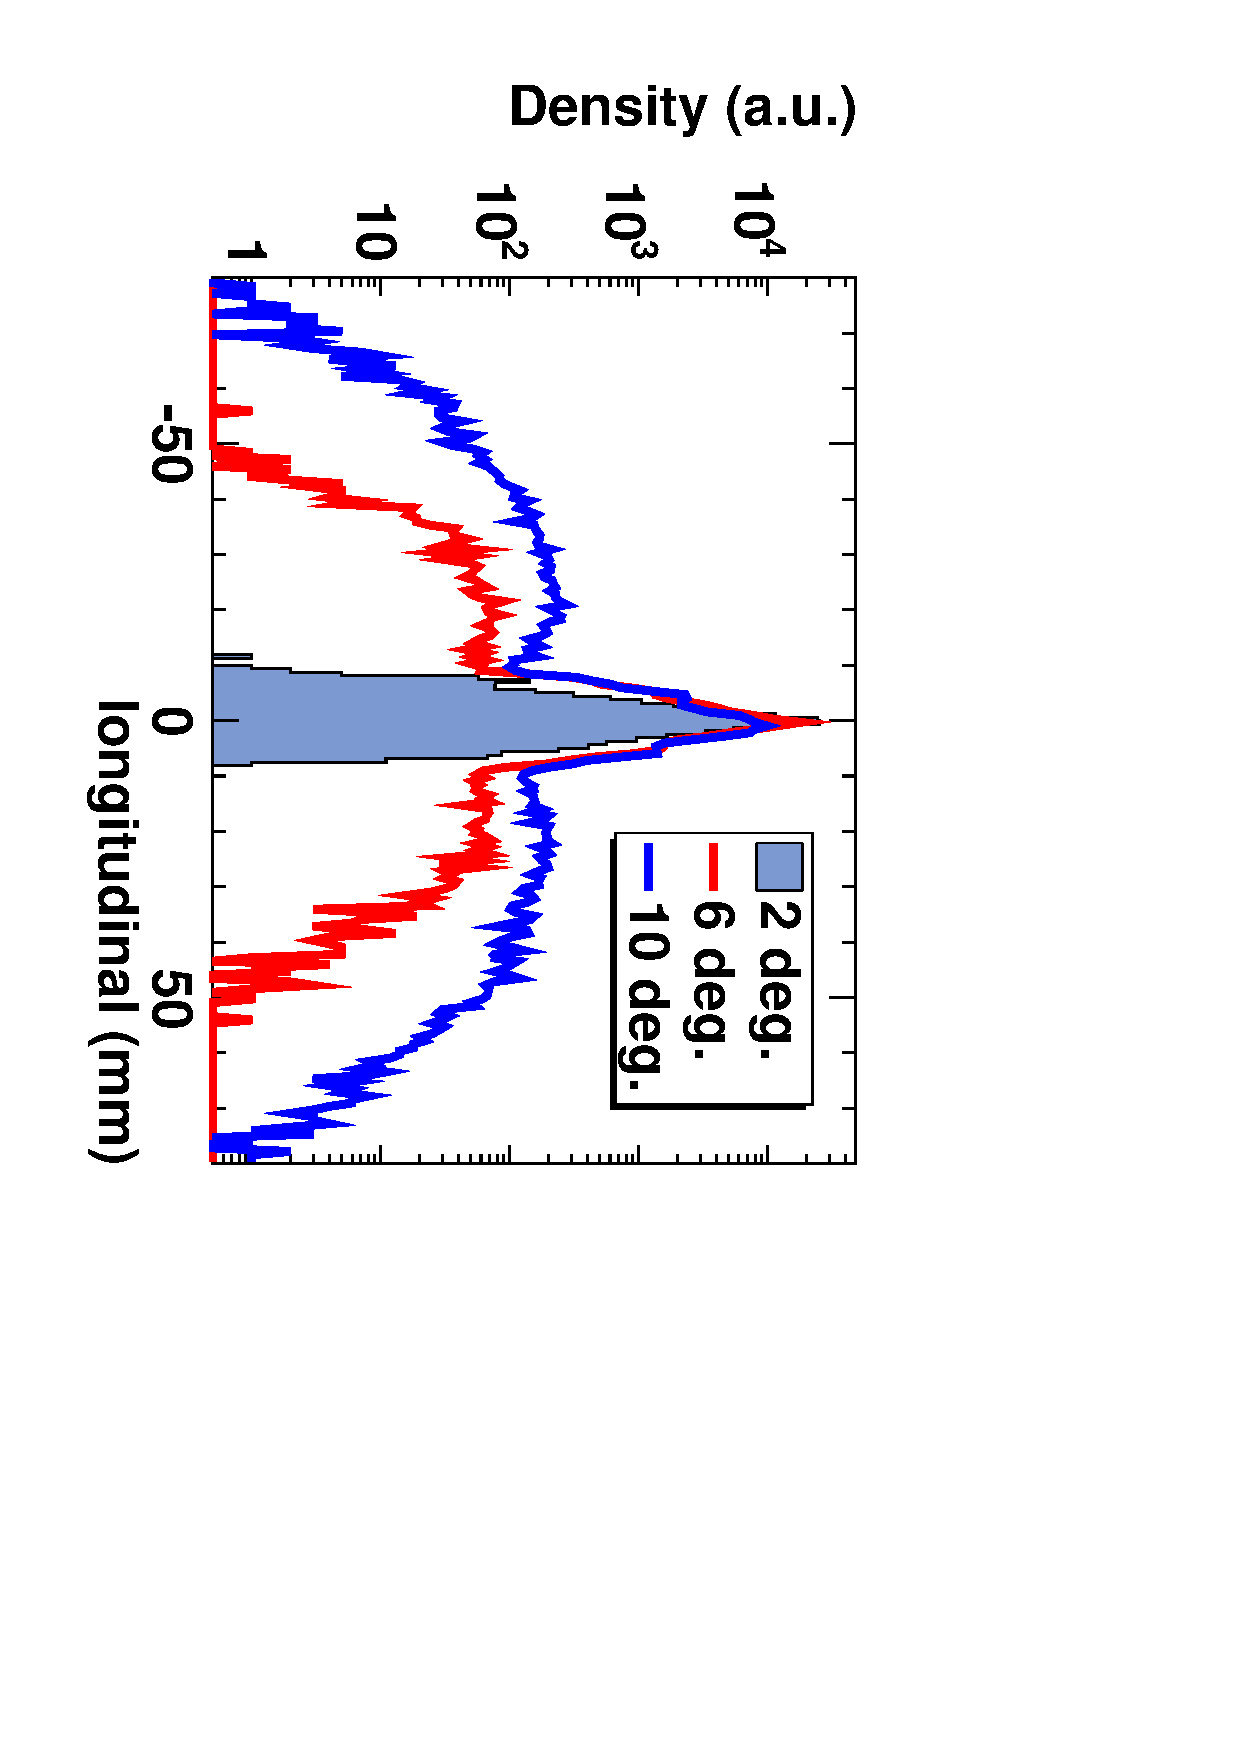
\includegraphics[angle=90,width=0.3\linewidth]{figures/Theta-Turn-150.pdf}
  \caption{Histogram of 3\,mA bunch distributions with  $2^o$, $6^o$ and $10^o$ initial phase widths at initial position(left),turn 50(middle) and 150(right) in PSI Ring cyclotron.}
  \label{fig:ThetaHitgram}
\end{figure*}

Fig.\,\ref{fig:RMSsize} shows the development of the beam rms size on the transverse and the longitudinal direction. We can see the beam is compressed
gradually in the longitudinal direction. Meanwhile in the transverse direction, the beam size increases fast during the first several turn 
because of the mismatch of initial conditions. Thereafter it does not change sufficiently until the beam arrives at the extraction region 
where it is distorted by the external magnetic field.
Fig.\,\ref{fig:RingPhaseWidth} shows the projection of phase space onto the middle plane of machine, and 
Fig.\,\ref{fig:ThetaHitgram} plots the histogram along the longitudinal direction at $112^o$ azimuthal position of turn 0, 50 and 150.
We can see for the bunch with the initial phase width of $2^o$, the bunch maintains very compact shape with a stable round core and no any haloes at all. 
When the initial phase width increases, the size of core only widens for less than 5\,mm, but the spiral tails expands in the longitudinal direction and 
can't develop stable haloes. However, the beam does not expands notably in radial direction, which means no substantial increase of the beam loss 
on the extraction septum is expected for the bunch with initial phase width less than $10^o$.

\subsection {Neighboring bunch effects in PSI Ring}

As discussed in section I, neighboring bunch effects may have appreciable influence on beam dynamics in the Ring. This can be evaluated by comparing the difference of single bunches simulation and multiple bunches simulation as describes in section III. We tested for 3, 5, 7 and 9 bunches and found that 
the difference between the center bunch of 7 scenarios and that of 9 bunches scenarios is trivial as shown in Fig.\,\ref{fig:NBcompare2D}. 
As we can see from Fig.\,\ref{fig:NBcompare}, the FWHD of beam transverse profile from multi-bunch simulation is 1\,mm narrower than that of single bunch and that the FWHD of energy spread is reduced slightly. This is caused by squeezing space charge force from the bunches at the smaller radius 
and those at the bigger radius. 

From the comparison, we conclude that neighboring bunch effects impose visible impacts on the beam dynamics when the beam current get beyond 1\,mA in PSI Ring. 
The bunch becomes more compact in the transverse direction and the energy spread is reduced slightly. Therefore neighboring bunch effects have positive influence
on reducing beam loss in high intensity operation.

\begin{figure*}
  \includegraphics[angle=90,width=1\linewidth]{figures/C9B7BSB-2D-1mA-130.pdf}
  \caption{Top view of 1\,mA bunch distributions at the turn 130  in the local frame ${\bs{S}_{local}}$ at $112^o$ azimuthal position of turn 130 in PSI Ring cyclotron.
    The results are obtained from single bunch(left), 7 bunches(middle) and 9 bunches(right) simulations, respectively.}
  \label{fig:NBcompare2D}
\end{figure*}

\begin{figure*}
  \includegraphics[angle=90,width=0.45\linewidth]{figures/C9B7BSB-R-1mA-130.pdf}
  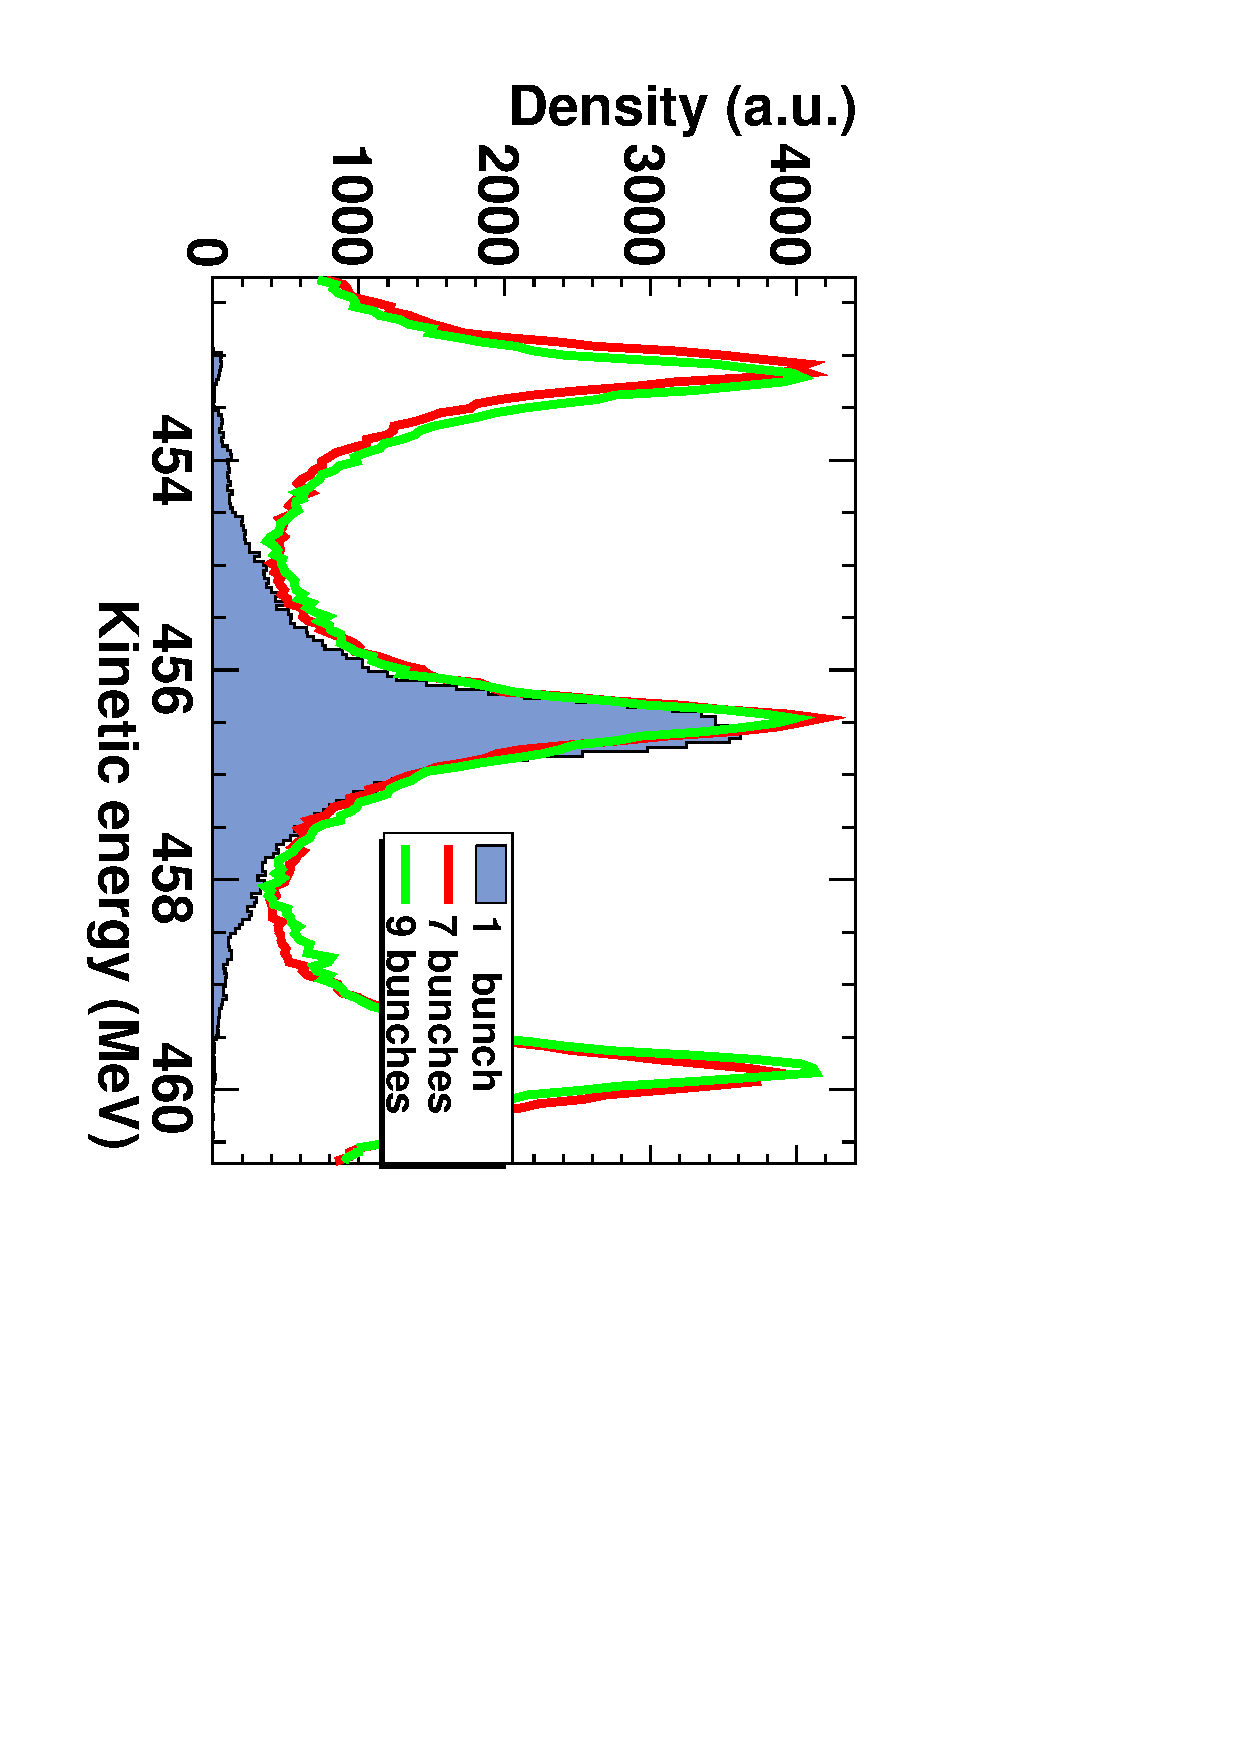
\includegraphics[angle=90,width=0.45\linewidth]{figures/C9B7BSB-Energy-1mA-130.pdf}
  \caption{Comparison of the histograms along the transferal direction in the local frame ${\bs{S}_{local}}$ (left) and the energy spectra (right) of 1\,mA beam
    at $112^o$ azimuthal position of turn 130 in PSI Ring cyclotron.}
  \label{fig:NBcompare}
\end{figure*}

\section{CONCLUSIONS AND DISCUSSIONS}
In this paper, we presented a physical model for the beam dynamics in high intensity cyclotrons, which includes for the first time the space charge effects
of neighboring bunches in a self-consistent way. This model is implemented in an object-oriented three-dimensional parallel PIC code, 
as a flavor of the \opal\, framework. 

The performance tests on CRAY XT3, CSCS show a good scalability of this code with the number of processors. 
The three working modes of this code were validated by comparison with other established codes. 

This code has been successfully applied to study the behavior of the PSI Ring cyclotron at high intensities.
As the results show, the generation of beam tails can be avoided if short bunches with a phase length of $2^o$  or less are injected. 
An upgrade plan is under way to generate such short bunches with the help of a 10$th$ harmonic buncher.
Furthermore it is observed that the neighboring bunch effects can help to narrow the transverse beam size and reduce the energy spread.

It is planned to refine these simulations within the next year by a more detailed determination of the initial particle distribution at the injection
of the PSI Ring cyclotron. A quantitative comparison of the results with measured beam properties will be presented in a future paper.
%Perform the first parallel simulation of multiple bunches in cyclotron
%Study neighboring bunch effects on the beam's evolution quantitatively on PSI Ring cyclotron
\section{ACKNOWLEDGMENTS}
The authors thank the AMAS grop members C.\,Kraus, Y.\,Ineichen and B.\,Oswald for many 
discussions regarding programming and T.\,Schietinger for providing the post-processing tool
H5PartRoot. We also thank Dr. W.\,Joho, S.\,Adam and R.\,Doelling for many useful discussions regarding high
intensity beam dynamics in cyclotrons. This work was performed on teh Merlin3 cluster at Paul Scherrer Institut 
and Cray XT3 at Swiss National Supercomputing Center (CSCS). 

% If in two-column mode, this environment will change to single-column
% format so that long equations can be displayed. Use
% sparingly.
%\begin{widetext}
% put long equation here
%\end{widetext}

% figures should be put into the text as floats.
% Use the graphics or graphicx packages (distributed with LaTeX2e)
% and the \includegraphics macro defined in those packages.
% See the LaTeX Graphics Companion by Michel Goosens, Sebastian Rahtz,
% and Frank Mittelbach for instance.
%
% Here is an example of the general form of a figure:
% Fill in the caption in the braces of the \caption{} command. Put the label
% that you will use with \ref{} command in the braces of the \label{} command.
% Use the figure* environment if the figure should span across the
% entire page. There is no need to do explicit centering.

% \begin{figure}
% \includegraphics{}%
% \caption{\label{}}
% \end{figure}

% Surround figure environment with turnpage environment for landscape
% figure
% \begin{turnpage}
% \begin{figure}
% \includegraphics{}%
% \caption{\label{}}
% \end{figure}
% \end{turnpage}

% tables should appear as floats within the text
%
% Here is an example of the general form of a table:
% Fill in the caption in the braces of the \caption{} command. Put the label
% that you will use with \ref{} command in the braces of the \label{} command.
% Insert the column specifiers (l, r, c, d, etc.) in the empty braces of the
% \begin{tabular}{} command.
% The ruledtabular enviroment adds doubled rules to table and sets a
% reasonable default table settings.
% Use the table* environment to get a full-width table in two-column
% Add \usepackage{longtable} and the longtable (or longtable*}
% environment for nicely formatted long tables. Or use the the [H]
% placement option to break a long table (with less control than 
% in longtable).
% \begin{table}%[H] add [H] placement to break table across pages
% \caption{\label{}}
% \begin{ruledtabular}
% \begin{tabular}{}
% Lines of table here ending with \\
% \end{tabular}
% \end{ruledtabular}
% \end{table}

% Surround table environment with turnpage environment for landscape
% table
% \begin{turnpage}
% \begin{table}
% \caption{\label{}}
% \begin{ruledtabular}
% \begin{tabular}{}
% \end{tabular}
% \end{ruledtabular}
% \end{table}
% \end{turnpage}

% Specify following sections are appendices. Use \appendix* if there
% only one appendix.
%\appendix
%\section{}

% If you have acknowledgments, this puts in the proper section head.
%\begin{acknowledgments}
% put your acknowledgments here.
%\end{acknowledgments}

% Create the reference section using BibTeX:
\bibliography{Refbase}

\end{document}
%
% ****** End of file template.aps ******

